\documentclass[11pt,fleqn]{article}
\usepackage{geometry} % see geometry.pdf on how to lay out the page. There's lots.
\geometry{a4paper} % or letter or a5paper or ... etc
% \geometry{landscape} % rotated page geometry
\usepackage{enumitem}

% See the ``Article customise'' template for come common customisations
\usepackage{times}
\usepackage{graphicx}
\usepackage{wrapfig}
\usepackage{xcolor}
\usepackage{url}
\usepackage{hyperref}
\usepackage{colortbl}
\usepackage{fancyhdr}
\usepackage{pdfpages}
\usepackage{pdflscape}
\usepackage{longtable}
\usepackage{arydshln}

% Notation as used in Robotics, Vision and Control textbook
%
% Shorthand and abbreviations
%   \hom -> homogeneous transform
%   \Hom -> Homogeneous transform
%   \etal
%   \eq{e} -> (e) which is a reference to equation e, eg. \ref{e}
%   \fnumber -> f-number
%   \Mlab -> MATLAB
%   \comma      comma + a short space
%   \tsub{k}   display timestep subscript in angle brackets <k>
%   \cspace  configuration space, curly C
%
% Linear algebra notation
% =================
%
%  A pre-superscript is used to indicate the reference coordinate frame.  This can be created using the macro
%
%  \presup{A}
%
% Points
% --------
%
%  Points are displayed in ???
%
%   \point[f]{P}
%   \coord{x}{y}    (x, y)
%
% Abstract pose
% ==========
%
% \pose          xi
% \estpose     xi with a hat
% \posedot     greek letter nu for spatial velocity
%
% \pose[R]          xi with a pre-superscript
% \estpose[R]     xi with a hat and a pre-superscript
% \posedot[R]     greek letter nu for spatial velocity with a pre-superscript
%
% Vectors
% ----------
%
% Vectors are displayed in bold italic font
%
%   \vec{x}     a vector
%   \vec[f]{x}  a vector with a coordinate frame
%
%   \dvec[f]{x}  a dotted vector 
%   \ddvec[f]{x}  a double dotted vector 
%   \vech[f]{x} a homogeneous vector (tilde above)
%   \vecb[f]{x} a vector with bar 
%   \tvec[f]{x} a homogeneous vector with a tilde
%   \hvec[f]{x} an estimated vector with a hat
%
%  if [f] not provided no presup is displayed
%
%
% Matrices
% -----------
%
%  Matrices are displayed in bold font
%
%   \mat{x}     a matrix
%   \mat[f]{x}  a matrix with a coordinate frame
%   \dmat[f]{x}  a matrix derivative
%   \sk{x}  -> S(x) skew symmetric matrix

% Quaternion
%
%   \q            a quaternion, q with a bubble on top
%
% Poses
%
%   \pose       pose
%   \estpose       estimated pose, with hat
%
%   \pose[f]    pose with respect to a frame
%   \pose        abstract pose
%   \posedot        derivative of abstract pose
%
% Lie Groups
% ========
%
% displayed in Roman font
%
%   \SO{n}   SO(n)
%   \SE{n}   SE(n)
%   \so{n}     so(n)
%   \se{n}     se(n)
%
% MATLAB code
% ===========
%
% Display a block of code in blue fixed-width font
%
%   \begin{Code}
%   \end{Code}
%
% other environments include
%   CodeSmall   uses a small font, useful for very wide lines
%   CodeNum    numbers the lines of code
%
% \var{} displays a variable in blue fixed-width font 
% \Mlab  displays MATLAB with the all letters bar the first in small caps font
%
% Units
% ====
% 
% Always set in Roman font with preceding thin space, can be used in math or LR mode.
%
%   \unit{}  eg. 20\unit{lx/m^2}.  
%   \Hz
%   \ms
%   \us   microseconds using mu
%   \nm
%   \deg  degrees shown with a bubble
%
% General shorthand notation
% =====================
%
%   \sci{5}{-2} format in scientific notation, 5 x 10^{-2}
%
%  \vector{x}{y}{z}    (x, y, z)
%  \comma  a comma followed by space
%  \cframe{a}  Coordinate frame {a}
%
%   \eq{ref}    reference an equation, in parentheses
%   \etal       et al.
%
%   \ba    begin eqnarray
%   \ea    end eqnarray
%
%   \hom    homogeneous transform
%   \Hom    Homogeneous transform
%
% Some common log-like functions
%
%   \floor
%   \ceil
%   \ord
%   \det
%   \trace  -> tr
%
%

\usepackage{amsmath, amssymb}

\usepackage{xifthen}
\usepackage{color}

\typeout{------ start of RVC notation ------}
\newcommand{\f}{f}

%

%
\renewcommand{\hom}{homogeneous transform}
\newcommand{\Hom}{Homogeneous transform}

\newcommand{\homeq}{\simeq}

\newcommand{\xstrut}[1]{\rule{0ex}{#1ex}}

\newcommand{\tsub}[1]{{\scriptstyle{\langle #1 \rangle}}}

\newcommand{\hstrut}{\rule{0mm}{7mm}}
\newcommand{\ba}{\begin{eqnarray}}
\newcommand{\ea}{\end{eqnarray}}

\newcommand{\eq}[1]{(\ref{#1})}
\newcommand{\etal}{{et al.}}
\newcommand{\fnumber}{\textit{f}-number}

%
% some common functions
%
%   \floor
%   \ceil
%   \ord
%   \det
%   \sk{}   skew symmetric matrix
\newcommand{\floor}{\mbox{floor}}
\newcommand{\ceil}{\mbox{ceil}}
\newcommand{\ord}{\mbox{Ord}}
\newcommand{\vex}{\mbox{vex}}

\renewcommand{\det}[1]{{\mbox{det}(\mat{#1})}}
\newcommand{\trace}[1]{{\mbox{tr}(\mat{#1})}}


%
% use as \sci{5}{-2} for formatting 5e-2
%
\newcommand{\sci}[2]{\mbox{$#1\!\cdot\!10^{#2}$}}


%
% macros to display units in math or LR mode, 20\unit{lx/m^2}
%
%   \unit{}
%   \Hz
%   \ms
%   \us
%   \deg
%
\newcommand{\unit}[1]{\mbox{$\mathrm{\,#1}$}}
\newcommand{\Hz}{\unit{Hz}}
\newcommand{\kHz}{\unit{Hz}}
\newcommand{\MHz}{\unit{Hz}}
\newcommand{\ms}{\unit{ms}}
\newcommand{\us}{\unit{\mu s}}
\renewcommand{\deg}{\mbox{${}^\circ$}}


\newcommand{\nm}{\unit{nm}}
\newcommand{\Dsixfive}{$\rm D_{65}$}

\newcommand{\R}{{\bf R}}
\newcommand{\zero}{{\bf 0}}

%
% notational shorthand (for consistency)
%   \q            a quaternion
%
%   \pose       pose
%   \pose[f]    pose with respect to a frame
%   \vec{x}     a vector
%   \vec[f]{x}  a vector with a coordinate frame
%   \dvec[f]{x}  a dotted vector with a coordinate frame
%   \ddvec[f]{x}  a double dotted vector with a coordinate frame
%   \vech{x}    a homogeneous vector
%   \vech[f]{x} a homogeneous vector with a coordinate frame
%   \vecb{x}    a vector with bar
%   \vecb[f]{x} a vector with bar and a coordinate frame
%   \hvec{x}    a vector with a hat
%
%   \mat{x}     a matrix
%   \mat[f]{x}  a matrix with a coordinate frame
%
%   \point[f]{P}
%   \frame[f]{P}{s}
%   \frameh[f]{P}{s}   \hat{P}
%   \frameb[f]{P}{s}   \bar{P}
%
%   \comma      comma + a short space
%   \coord{x}{y}    (x, y)
%   \vector{x}{y}{z}    (x, y, z)
%  \pose        abstract pose
%  \posedot        derivative of abstract pose
\newcommand{\im}[1]{\mathbf{#1}}
\newcommand{\presup}[1]{\,{}^{\scriptscriptstyle #1}\!}
\newcommand{\relval}[2]{\presup{#1}{#2}}
\newcommand{\pose}[1][ZZZZ]{\ifthenelse{\equal{#1}{ZZZZ}}{}{\presup{#1}}{\mathbf{\xi}}}
\newcommand{\estpose}[1][ZZZZ]{\ifthenelse{\equal{#1}{ZZZZ}}{}{\presup{#1}}{\mathbf{\hat{\xi}}}}
\newcommand{\hpose}[1][ZZZZ]{\ifthenelse{\equal{#1}{ZZZZ}}{}{\presup{#1}}{\hat{\mathbf{\xi}}}}
\newcommand{\posedot}[1][ZZZZ]{\ifthenelse{\equal{#1}{ZZZZ}}{}{\presup{#1}}{\mathbf{\nu}}}


\newcommand{\q}{\mathring{q}}

\DeclareMathAlphabet{\mathitbf}{OML}{cmm}{b}{it}
\newcommand{\twist}[2][ZZZZ]{\ifthenelse{\equal{#1}{ZZZZ}}{}{\presup{#1}}{\mathcal{S}}}
\renewcommand{\vec}[2][ZZZZ]{\ifthenelse{\equal{#1}{ZZZZ}}{}{\presup{#1}}{\mathitbf{#2}}}

\newcommand{\hvec}[2][ZZZZ]{\ifthenelse{\equal{#1}{ZZZZ}}{}{\presup{#1}}{\hat{\vec{#2}}}}
\newcommand{\tvec}[2][ZZZZ]{\ifthenelse{\equal{#1}{ZZZZ}}{}{\presup{#1}}{\tilde{\vec{#2}}}}
\newcommand{\evec}[2][ZZZZ]{\ifthenelse{\equal{#1}{ZZZZ}}{}{\presup{#1}}{\hat{\vec{#2}}}}
%
\newcommand{\dvec}[2][ZZZZ]{\ifthenelse{\equal{#1}{ZZZZ}}{}{\presup{#1}}{\dot{\vec{#2}}}}
\newcommand{\ddvec}[2][ZZZZ]{\ifthenelse{\equal{#1}{ZZZZ}}{}{\presup{#1}}{\ddot{\vec{#2}}}}

\newcommand{\hv}[1]{\ensuremath{\stackrel{\textstyle{#1}}{\textstyle{\sim}}}}
\newcommand{\vech}[2][ZZZZ]{\ifthenelse{\equal{#1}{ZZZZ}}{}{\presup{#1}}{\mathitbf{\tilde{#2}}}}
\newcommand{\vecb}[2][ZZZZ]{\ifthenelse{\equal{#1}{ZZZZ}}{}{\presup{#1}}{\bar{\underline #2}}}
\newcommand{\mat}[2][ZZZZ]{\ifthenelse{\equal{#1}{ZZZZ}}{}{\presup{#1}\,}{{\boldsymbol #2}}}
\newcommand{\hmat}[2][ZZZZ]{\ifthenelse{\equal{#1}{ZZZZ}}{}{\presup{#1}\,}{{\hat{\boldsymbol #2}}}}
\newcommand{\dmat}[2][ZZZZ]{\ifthenelse{\equal{#1}{ZZZZ}}{}{\presup{#1}\,}{{\dot{\boldsymbol #2}}}}
\newcommand{\emat}[2][ZZZZ]{\ifthenelse{\equal{#1}{ZZZZ}}{}{\presup{#1}\,}{\hat{\boldsymbol #2}}}
\newcommand{\matfn}[3][ZZZZ]{\ifthenelse{\equal{#1}{ZZZZ}}{}{\presup{#1}}{{\mat{#2}}\left(#3\right)}}
\newcommand{\Rt}[2][ZZZZ]{\ifthenelse{\equal{#1}{ZZZZ}}{}{\presup{#1}}{{\bf R}\left(#2\right)}}


%\newcommand{\homt}[3]{{}^{#1}{\bf #3}_{#2}}
%\renewcommand{\frame}[2]{{}^{#1}{#2}}

\newcommand{\cframe}[1]{\{#1\}}
\newcommand{\cspace}{{\cal C}}
\newcommand{\point}[2][ZZZZ]{\ifthenelse{\equal{#1}{ZZZZ}}{}{\presup{#1}}{\mathbf{\mathrm{#2}}}}

\newcommand{\comma}{,\;}
\newcommand{\coord}[2]{\left( #1 \comma #2 \right)}
\renewcommand{\vector}[3]{\left( #1 \comma #2 \comma #3 \right)}



% Matlab documentation macros
\newfont{\School}{pncr}
\newfont{\eightTR}{pncr at 8pt}
%\newfont{\vtt}{pcrr}

\newcommand{\fullstop}{\,\,\,.}
\newcommand{\termsep}{\,\,\,,}
\typeout{------ end of notation ------}

\newcommand{\del}[1]{\delta_{#1}}
\newcommand{\vdel}[1]{\vec{\delta}_{#1}}

%=====================================================================
%  MATLAB code support
%=====================================================================

\usepackage{color}
% Matlab code example environment
%   for code examples.
%   each executable line must begin with >>
%   comments start with !
%   lines starting !>> are executed during parsing, but dont print
%   
%   \begin{Code}
%   \end{Code}
\usepackage{fancyvrb}
\fvset{formatcom=\color{blue},fontseries=c,fontfamily=courier,xleftmargin=4mm,commentchar=!}

\DefineVerbatimEnvironment{Code}{Verbatim}{formatcom=\color{blue},fontseries=c,fontfamily=courier,fontsize=\footnotesize,xleftmargin=4mm,commentchar=!}

\DefineVerbatimEnvironment{CodeSmall}{Verbatim}{formatcom=\color{blue},fontseries=c,fontfamily=courier,fontsize=\scriptsize,xleftmargin=1mm,commentchar=!}

\DefineVerbatimEnvironment{CodeNum}{Verbatim}{numbers=left,numbersep=4pt,formatcom=\color{blue},fontseries=c,fontfamily=courier,fontsize=\footnotesize,xleftmargin=4mm}

%\var{}
%\Mlab

\newcommand{\var}[1]{{\color{blue}\Verb+#1+}}
\newcommand{\model}[1]{\index{code}{#1@\textit{#1}}\ifthenelse{\boolean{draft}}{{\color{green}\Verb+#1+}}{\Verb+#1+}}
\newcommand{\block}[1]{\ifthenelse{\boolean{draft}}{{\color{green}\Verb+#1+}}{\textsf{#1}}}

%\newcommand{\func}[1]{{\color{blue}\Verb+#1+}}
\newcommand{\func}[2][ZZZZ]{\ifthenelse{\equal{#1}{ZZZZ}}{\index{code}{#2}}{\index{code}{#1}}\ifthenelse{\boolean{draft}}{{\color{green}\Verb+#2+}}{\Verb+#2+}}

\newcommand{\methodb}[2]{\index{code}{#1@\textbf{#1}!.#2}\ifthenelse{\boolean{draft}}{{\color{magenta}\Verb+#1.#2+}}{\Verb+#1.#2+}}
\newcommand{\method}[2]{\index{code}{#1@\textbf{#1}!.#2}\ifthenelse{\boolean{draft}}{{\color{magenta}\Verb+#2+}}{\Verb+#2+}}
\newcommand{\class}[1]{\index{code}{#1@\textbf{#1}}\ifthenelse{\boolean{draft}}{{\color{cyan}\Verb+#1+}}{\Verb+#1+}}
\newcommand{\property}[1]{\index{property}{#1}\ifthenelse{\boolean{draft}}{{\color{cyan}\Verb+#1+}}{\Verb+#1+}}

%\newcommand{\Mlab}{{M\textsc{ATLAB}}}
\newcommand{\MATLAB}{MATLAB\textsuperscript{\textregistered}}

\newcommand{\SE}[1]{\ensuremath{\mathrm{{\bf SE}(#1)}}}
\newcommand{\SO}[1]{\ensuremath{\mathrm{{\bf SO}(#1)}}}
\newcommand{\se}[1]{\ensuremath{\mathrm{{\bf se}(#1)}}}
\newcommand{\so}[1]{\ensuremath{\mathrm{{\bf so}(#1)}}}
\newcommand{\isk}[1]{\vee\left( #1\right)}
\newcommand{\iskx}[1]{\vee_{\times}\left( #1\right)}
\newcommand{\skx}[1]{\left[#1\right]_{\times}}
\newcommand{\sk}[1]{\left[#1\right]}
%\newcommand{\norm}[1]{\Vert #1 \Vert}
\newcommand{\Ad}{\mbox{Ad}}
\newcommand{\ad}{\mbox{ad}}



\setlength{\parindent}{0pt}
\newcommand{\IDX}[1]{\textbf{\textcolor{red}{#1}}}
\newcommand{\SIDENOTE}[1]{\textbf{\textcolor{blue}{#1}}}
\newcommand{\rpi}{Raspberry Pi}

\title{A mobile robot for education: the PenguinPi}
\author{Peter Corke}
\date{July 2018} % delete this line to display the current date

\makeatletter
           \let\Date\@date
\makeatother

%%% BEGIN DOCUMENT
\begin{document}
\maketitle
\pagestyle{fancyplain}
%\pagestyle{headings}        % Gives page headings at top of page
\rfoot{Revision of \Date }
%\rfoot{Copyright \copyright Peter Corke \rtbyear}


This report describes a low-cost mobile robot  designed for robotics education.
The teaching objectives are described and this leads to a specification for the robot.
The remainder of the report provides a detailed technical description of the Penguin Pi  robot and its implementation.

\begin{figure}[h]
\centering
\includegraphics[width=14cm]{P1080377.JPG}
%\caption{The Mark II Penguin Pi robot}\label{fig:robot}
\end{figure}

\newpage
\tableofcontents
\newpage

%%%%%%%%%%%%%%%%%%%%%%%%%%%%% INTRODUCTION
\section{Educational objectives}

The mobile robotics learning outcomes we wish to achieve include:
\begin{enumerate}
\item Motion models: how configuration (pose) of the robot evolves with time for key types of platform such as Ackerman steering and differential steering.
\item Motion control: how to design a controller that will move the robot from an initial to a desired final configuration, or to follow a path.  
Initially we will assume that robot configuration is measured (externally) and provided as input to the robot controller.
\item Motion planning: how to find a path to move from A to B
\begin{enumerate}
  \item For a grid-based map that denotes occupied and free space, how to plan an obstacle-free path using the distance transform (aka wavefront or grass fire) algorithm
  \item For a graph-based map using breadth-first, uniform-cost, A* search, or D* algorithms to find an optimal path.
\end{enumerate}
\item Robot localization: how to use observations of known landmarks to estimate robot configuration (``where am I?'').
\item Map making: how to convert landmark observations into a consistent estimated map  assuming that robot configuration is known.
\item Simultaneous localization and mapping: how to create a map and estimate robot configuration based on observations of initially unknown landmarks.
\end{enumerate}

\section{Robot specification}
To explore these learning principles, we require a robot with the ability to move, to report its motion (odometry), to observe landmarks, and make use of an external sensor that reports the robot's configuration.

The robot requires the following features to support these learning outcomes:
\begin{enumerate}
\item Differential-drive platform which is very general.  While quite simple and low-cost to fabricate, 
a software emulation can convert this platform to a virtual Ackerman-steered configuration (the reverse is not true).  
\item A means to provide odometry which is required to estimate current configuration.  Options include:
\begin{enumerate}
  \item Wheel encoders to provide incremental wheel rotation. Ideally these would be quadrature but if motion is in only one direction it could be a simpler and cheaper non-quadrature encoder.
  \item An optical mouse chip to measure x- and y-axis displacement of a point on the robot relative to the ground.  %The ADNS2620 was ideal but now obsolete and there is no obvious replacement.
\end{enumerate}

\item Camera to observe landmarks for localization or visual odometry.  There are many options and the choice could be part of the
student's exercise. Options include:
\begin{enumerate}
  \item Front-mounted forward-looking perspective camera with a limited field of view.
  \item A $360^\circ$ panoramic camera, and there are some low-cost options such as the \href{https://www.robotshop.com/en/arducam-arduino-panorama-360-shield.html?gclid=CjwKCAjwzenbBRB3EiwAItS-u6KTmb5BQqjRGf7BO9a-Hu-UunogtEtZXQYSLflw6E3C5bTaU5SCERoCFZEQAvD_BwE}{ArduCAM (based on 4 regular cameras}.
  \item  An upward-facing \href{https://www.raspberrypi.org/magpi/building-a-raspberry-pi-360-camera/}{catadioptric camera using a low-cost iPhone camera adaptor}.
\end{enumerate}

\item Battery and a means to charge it, ideally while the battery is connected to the robot and the robot is powered up.  Also the
ability to monitor battery voltage.
  \item WiFi communications for tether-less operation. Ideally able to work in the university lab, a student's home or even act as a wireless access point to allow operations in areas with no WiFi infrastructure.

\item An external localization service to provide an estimate of the robot's pose as an input to a motion controller.  This capability will be used initially until students have mastered the techniques to perform localization themselves.  After that, the external localization can be used to provide a ground truth for comparison purposes.  Some options for an external localizer include:
\begin{enumerate}
\item Dead reckoning based on wheel encoders, implemented onboard the robot at a relatively high sample rate.
\item An overhead camera, looking down at distinctive visual markers/beacons on the robot, possibly infra-red (IR) LEDs.
\item A camera on the robot looking up at specialized markers on the ceiling, for example the \href{https://github.com/gestom/whycon-orig.git}{WhyCon system}.
\item Two IR receivers working with one (maybe two) \href{https://en.wikipedia.org/wiki/HTC_Vive}{HTC/Valve Vive base stations} which scan planes of IR light across the workspace.
\end{enumerate}

\item Convenient programming environment for code running either onboard or offboard the robot.  In either case it would be useful to have graphical display of the robot's state and its perceived environment.  For code running offboard the robot, communications latency is likely to be an issue.
Possible programming paradigms include:
\begin{enumerate}
\item Student MATLAB running offboard and communicating via a simple API with provided software running on the  robot 
\item Student Python code running onboard using a Python API
\item Student MATLAB code running in MATLAB Online (in the cloud so no need for a local MATLAB instance) communicating via a simple API with either the low-level robot hardware or provided software running on the robot 
\item Student MATLAB code, using a simple API, compiled to C code and running onboard the robot.
\end{enumerate}

\end{enumerate}

%%%%%%%%%%%%%%%%%%%%%%%%%%%%% ROBOT COMPUTE
\section{The PenguinPi robot}
The robot is shown in Figure \ref{fig:robot-annotated}.
It was developed as a final year student project by Jack Wright in 2016.
Jack was also a student of the EGB439 Advanced Robotics
unit, which at that time used Lego Mindstorm for the practical work.
The robot was refined by Jack and Steven Bulmer over the summer of 2016/7 and the Mark I was used for
the class in 2017 and for a workshop at the Robotic Vision Summer School in early 2018.
A Mark II version was developed over the summer of 2017/8 and used for  class in first semester of 2018.
In the second half of 2018 the onboard software was substantially refactored and extended.


\subsection{Computing systems}
The main processor is a Raspberry Pi 3B with an attached camera (PiCam). 
It includes a microSD card slot, four USB ports, built in BlueTooth and WiFi and an HDMI port and a 40-pin expansion connector.
The operating system is Rasberian and includes python and OpenCV.  ROS is not pre-installed.
By connecting an HDMI monitor plus USB keyboard and mouse the Raspberry Pi provides a capable standalone Linux system with windowed desktop environment.
For mobile operation we use WiFi and connect to it using \texttt{ssh} or web services.
We prefer a 5\unit{GHz} USB dongle over the onboard 2.4\unit{GHz} WiFi capability to avoid congestion in lab sessions with many 
robots.

\begin{figure}
\centering
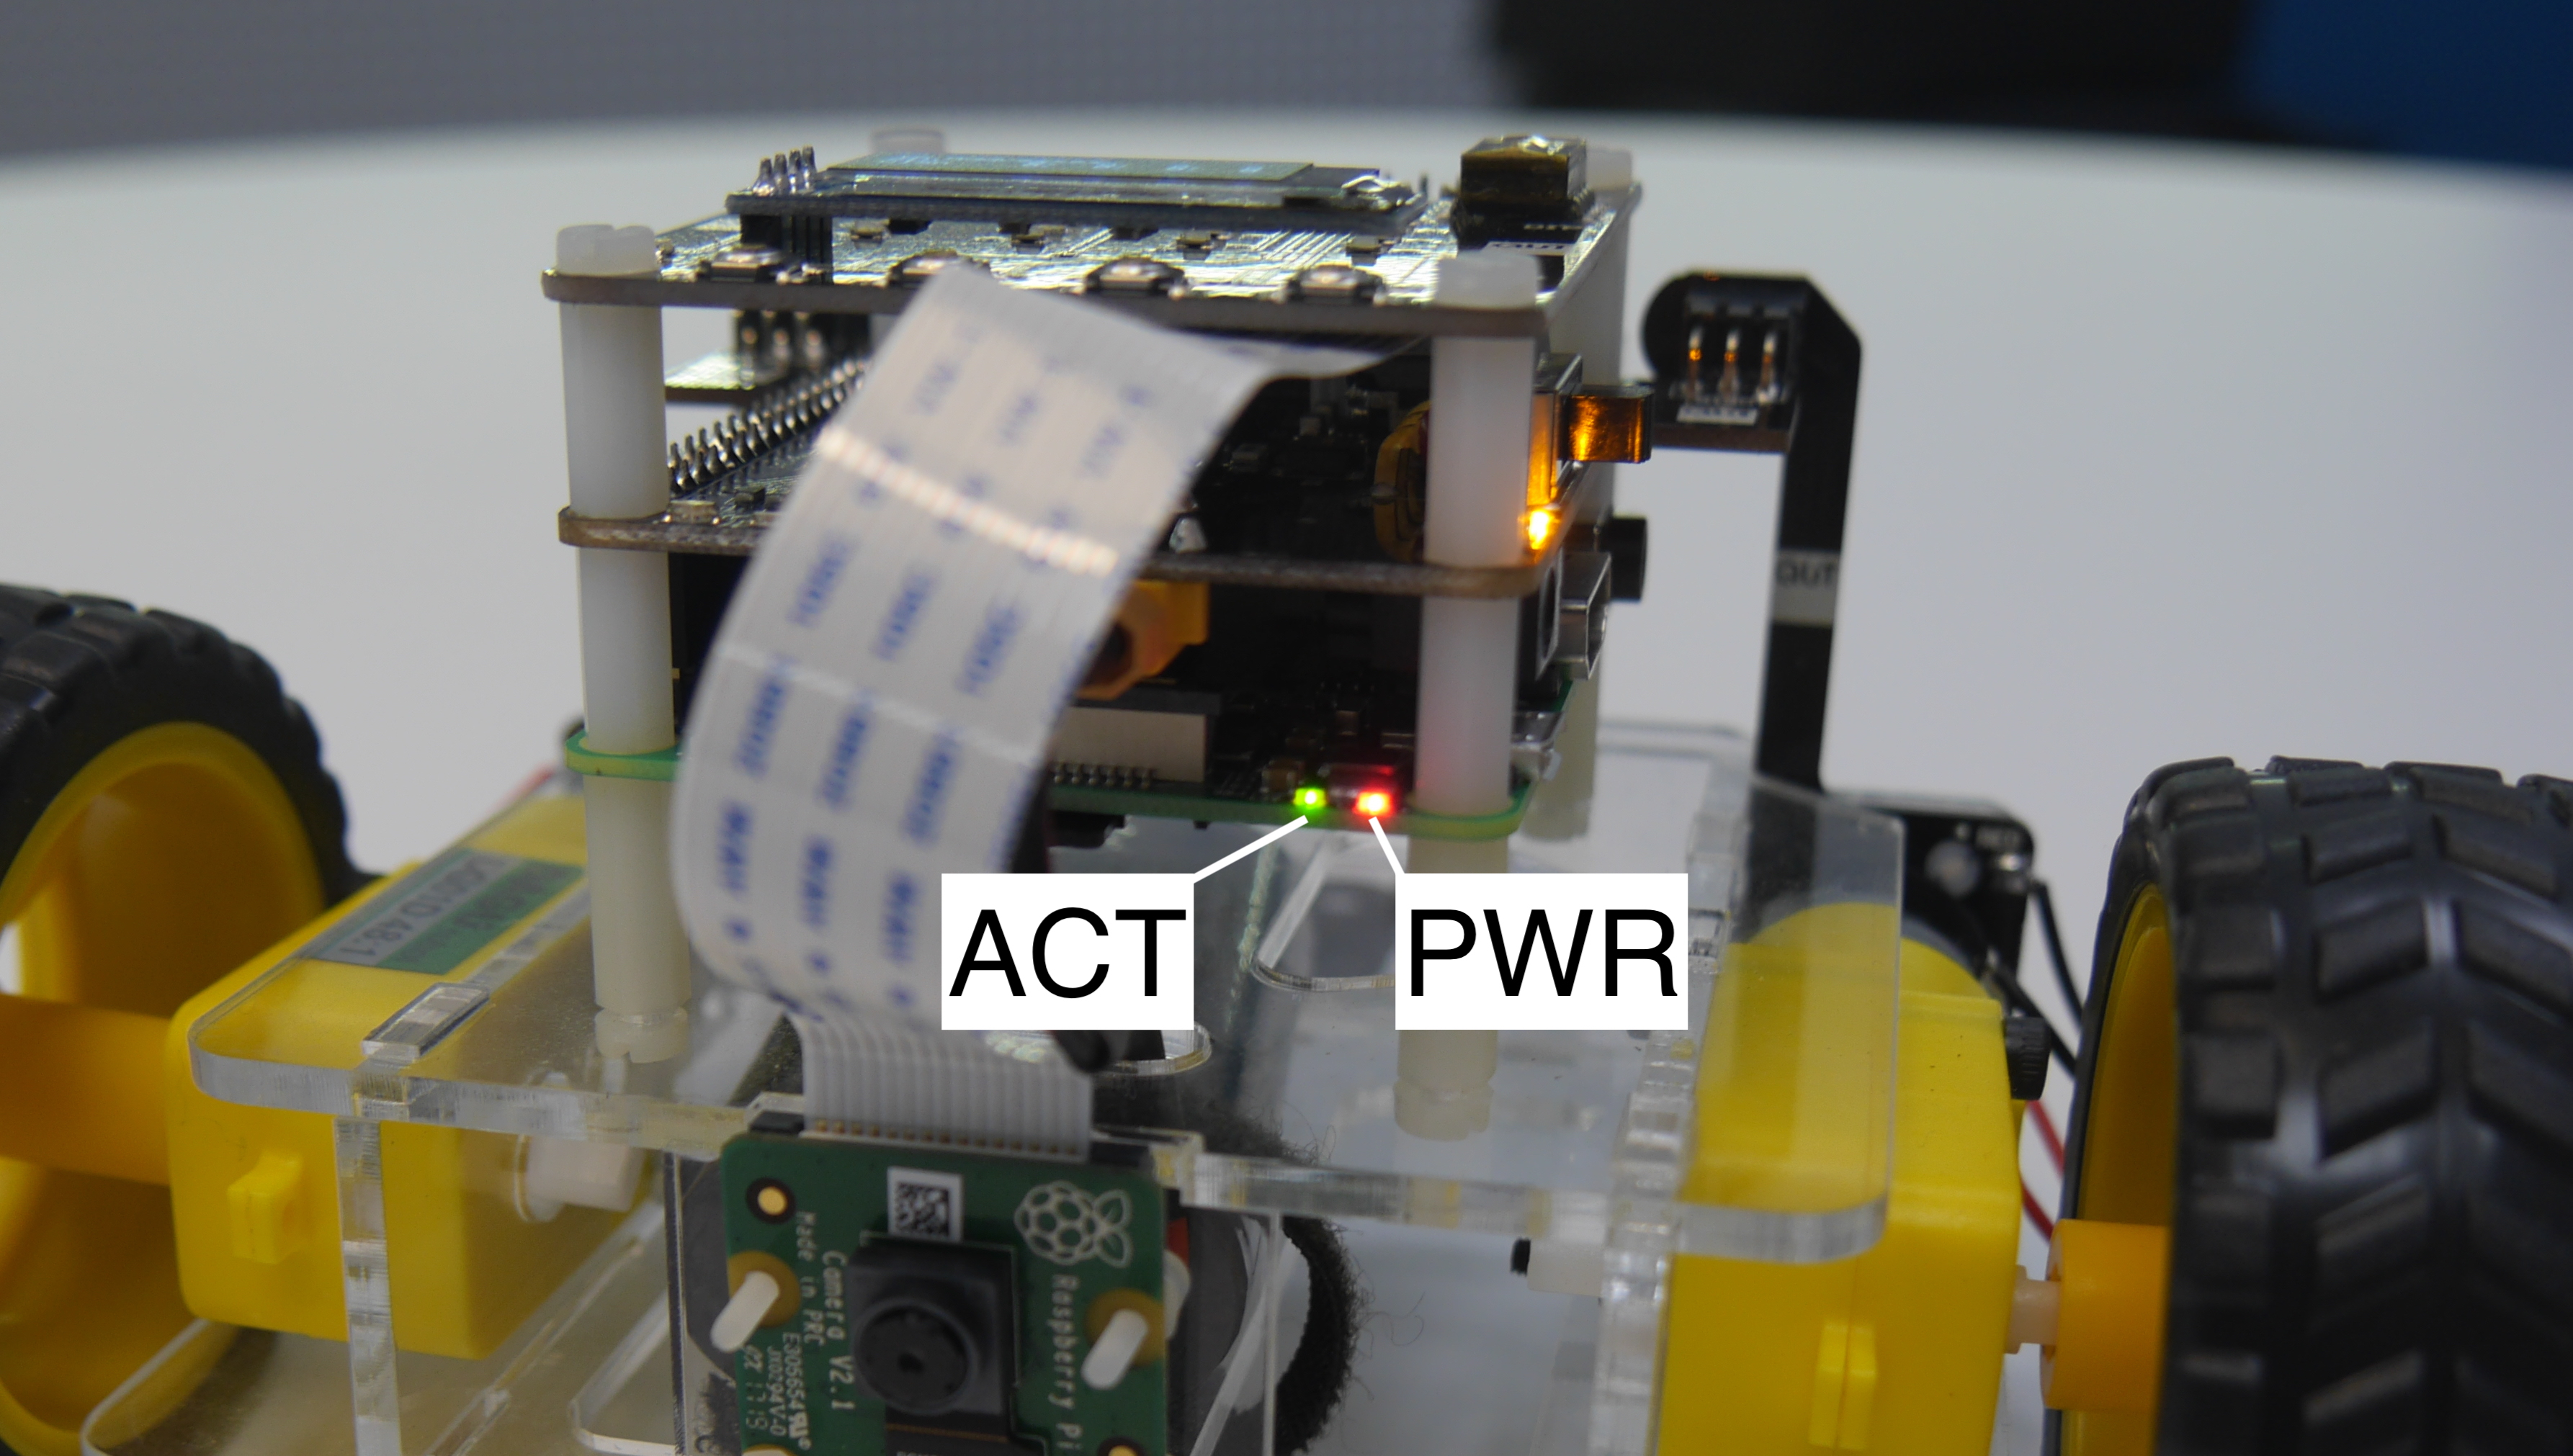
\includegraphics[width=10cm]{P1080367.JPG}
\caption{Raspberry Pi LED indicators}\label{fig:pi-leds}
\end{figure}

The Raspberry Pi 3B has two LEDs to the right of the microSD card slot shown in Fig \ref{fig:pi-leds}:
\begin{itemize}
\item ACT (green) indicates that the SD card is being read or written.  A repetitive pattern of flashes at startup indicates issues
with the SD card or boot process;
\item PWR (red) indicates that the board is powered (it will flash for voltage below 4.63\unit{V}).
\end{itemize}

Alternative computer platforms would include:
\begin{itemize}
\item  BeagleBone Blue, but by comparison  the Raspberry Pi 3 has several key advantages:
 half the cost, has a low-cost camera and interface, and is easy to expand for i/o without needing specialised cables.
\item  Libre computer Le Potato or Renegade
\end{itemize}

The PenguinPi daughter board (PPI) is a Raspberry Pi expansion board that attaches to the Pi's 40-pin expansion connector.
It contains an Atmel 644 8-bit processor with 64k program space and 4k of RAM.  It performs motor control, power management and supports a simple user interface (UI), has a number of indicator LEDs.
It can be expanded by an additional ``hat'' board.
One such board -- HAT1 -- provides infra-red beacon LEDs and a simple user interface comprising push buttons and a small OLED display.

The RaspberryPi and the PPI processors communicate over a high-speed serial port for message exchange, error diagnostics (from the PPI) and display of text strings on the OLED display.

\begin{figure}
\centering
\includegraphics[width=15cm]{montage-annotated.pdf}
\caption{Annotated view of the Penguin Pi robot}\label{fig:robot-annotated}
\end{figure}

%%%%%%%%%%%%%%%%%%%%%%%%%%%%% ROBOT HARDWARE
\subsection{Robot hardware}
\subsubsection{Motors}
The robot is driven by a pair of ROB-13302 brushed permanent-magnet DC gearmotors with a right-angle gearbox and a reduction ratio of 48:1.  Specifications are:
\begin{itemize}
\item voltage 4.5\unit{V}
\item no load maximum speed of 140\,RPM
\item no load current 190\unit{mA}, this is effectively the Coulomb friction torque
\item maximum load current 250\unit{mA}
\item maximum torque 800\unit{gf \cdot cm} or $0.8 \times 9.81 \times 0.01 =  78.4\unit{mN}$. 
If this is the nett torque \textit{after} friction, then  the torque constant (including gearbox) is $78.4/(250-190) =1.31\unit{N \cdot m/A}$.
The back EMF constant would therefore be 1.31\unit{V\cdot s/rad}.
\end{itemize}

The wheels are ROB-13259 with a diameter of $D=65\unit{mm}$.

\begin{figure}
\centering
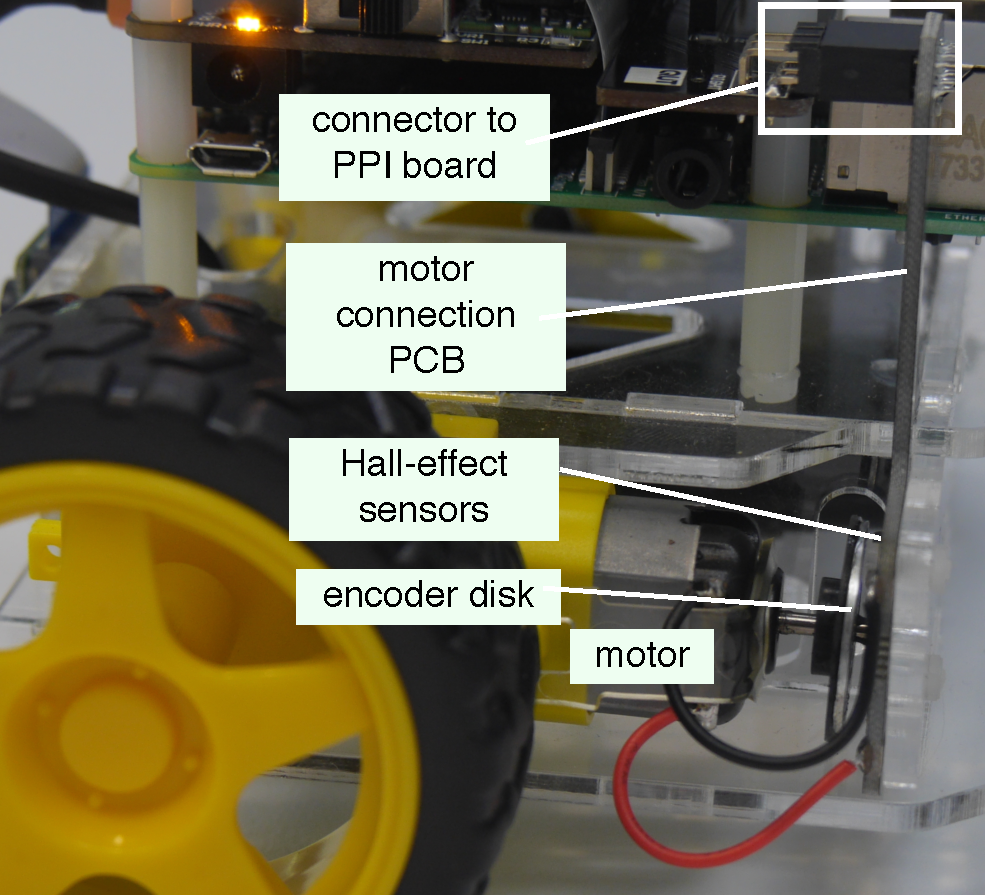
\includegraphics[width=12cm]{motor-annotated.pdf}
\caption{Closeup view the Penguin Pi robot showing the motor, the encoder disk and the PCB which holds the Hall-effect sensors, and 
which plugs into the PPI board.}\label{fig:robot-closeup}
\end{figure}

The motor shaft, before the gearbox, is fitted with an ROB-12629 encoder disk which has 8  poles (4 north poles and 4 south poles) which can be
seen in Figure \ref{fig:robot-closeup}.


\subsubsection{Motor speed response}\label{sec:motor-control}

The response of the motor to applied voltage (percentage of maximum PWM) is shown in Figure \ref{fig:motor-response}. 
It fits well to a line through the origin with a slope of 11.5 but at command below 30 the effect of friction becomes
evident, with no motion for a command of 9 or less.
The maximum encoder rate is 1100\unit{enc/s} or 2.87\unit{rev/s} which is approximately 25\% higher than the motor's rated speed
of 140\,RPM or 2.33\unit{rev/s} -- perhaps indicating that the maximum applied voltage is higher than the motor's specified maximum.

\begin{figure}
\centering
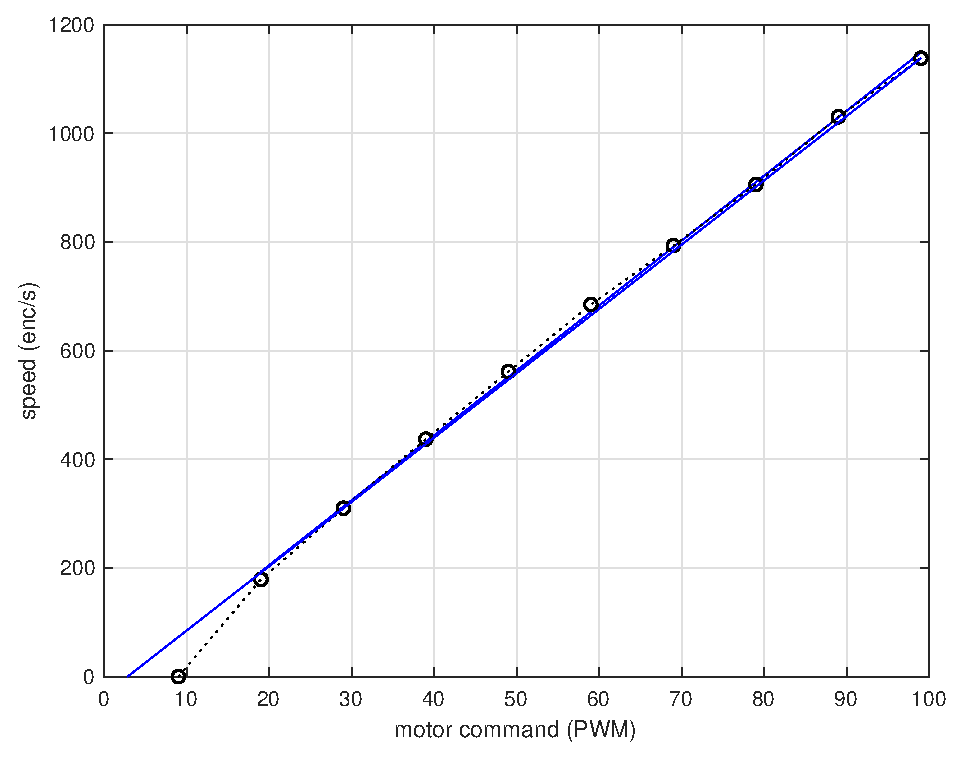
\includegraphics[width=8cm]{motor.eps}
\caption{Open-loop motor response to applied PWM voltage (percentage) for motor A.}
\label{fig:motor-response}
\end{figure}

Ignoring motor inductance  we can write motor current as
\begin{equation}
i = \frac{V - V_b}{R} \label{eq:current}
\end{equation}
where $R$ is motor armature resistance and
\begin{equation}
V_b = K_b \varpi \label{eq:bemf}
\end{equation}
is the back EMF where $K_b$ is the back EMF constant.
Nett motor torque is
\begin{equation}
\tau = \left\{ \begin{array}{ll} 0 & |K_\tau i| \le \tau_C \\ K_\tau i - B\varpi - \mathrm{sgn}(\varpi )\tau_C & |K_\tau i| > \tau_C \end{array} \right. \label{eq:torque}
\end{equation}
where $B$ is viscous friction, $\tau_C$ is Coulomb friction (assumed symmetric) and $K_\tau$ is the motor torque constant.

While moving at steady state, nett torque $\tau = 0$, we can substitute \eq{eq:current} and \eq{eq:bemf} into \eq{eq:torque} to obtain
\begin{equation*}
K_\tau \frac{V - K_b \varpi}{R} - B\varpi - \tau_C = 0
\end{equation*}
and simplifying with $K = K_b = K_\tau$ then
\begin{equation}
\varpi = \frac{K V - \tau_C R}{K^2 + BR} = V \frac{K}{K^2 + BR} -   \frac{\tau_C R}{K^2 + BR}
\end{equation}
which is similar in appearance to Figure \ref{fig:motor-response}.  From the slope (11.95) and breakpoint (-33.74) , and assuming knowledge of $K$ and $\tau_C$ from above, we could estimate $R$ and $B$.

The resulting motor speed ignores disturbance torque from wheel-ground interaction which will be highly dependent on the ground material and  be significant during skid steering.  To overcome this a motor velocity controller can be enabled by setting switch 4 of the DIP switch to ON.
It may be possible to estimate  friction characteristics from the measured battery current.

%%%%%%%%%%%%%%%%%%%%%%%%%%%%%%%%%%%%%%%%%%%%%%%%%%%%%%
%%%%%%%%%%%%%%%%%%%%%%%%%%%%%%%%%%%%%%%%%%%%%%%%%%%%%%
\subsection{Penguin Pi expansion board (PPI)}
The Penguin Pi (PPI) is a small circuit board that connects to the Raspberry Pi GPIO connector.  
It manages a LiPo battery, drives the motors, and interfaces with motors, encoders and a number of LEDs.

\subsubsection{Encoders}

The sensor is an \href{https://www.google.com/url?sa=t&rct=j&q=&esrc=s&source=web&cd=2&ved=2ahUKEwie-sPD3pzdAhUPVt8KHQ58Ad0QFjABegQICRAC&url=https%3A%2F%2Fwww.allegromicro.com%2F~%2Fmedia%2FFiles%2FDatasheets%2FA112x-Datasheet.ashx&usg=AOvVaw0f7rcuUrchXBUwaIueUS9B}{Allegro A1120 unipolar Hall-effect sensor} which turns on when it sense a magnetic south pole.
The motor shaft is fitted with an ROB-12629 encoder disk which has 8  poles (4 north poles and 4 south poles), so the sensor output will have four on-periods and four off-periods per shaft revolution.
The processor is configured to interrupt on changes to the encoder signal (rising and falling edges) of which there are
eight per revolution.  Given the 48:1 gearbox ratio there will be $48 \times 8 = 384$ encoder interrupts per wheel revolution.

The encoder, and the encoder sensing board can be
seen in Figure \ref{fig:robot-closeup}.  This board, which connects to the main PPI board eliminates a lot of point-to-point wiring which 
 led to high build time and poor reliability with the Mark 1 robot.




%%%%%%%%%%%%%%%%%%%%%%%%%%%%% SPEED CONTROL
\subsubsection{Motor driver}\label{sec:motor-control}
The motor voltages are controlled via 8-bit PWM motor drivers with values in the range 0 to 255.
This is performed by Timer 0 and the output compare registers OCR0A and OCR0B.
Motor direction, or applied polarity, is controlled by digital outputs PB0 and PB1 respectively.

 The software considers motor commands in the range -100 to +100 are these are mapped to PWM settings in the range 0-255 plus motor direction.


\subsubsection{Atmel clocks and timing}
The processor has a 20\unit{MHz} external crystal connected between pins XTAL1 and XTAL2.  
The clk$_{\mbox{I/O}}$ signal (20\unit{MHz}) from the clock control logic is used for all timers.  
The clk$_{\mbox{I/O}}$ signal is controlled
by the:
\begin{itemize}
\item Clock source multiplexer, which is set to external crystal oscillator (CKSEL bits in the \texttt{lfuse} fuse byte)
\item System clock prescaler is bypassed, ie. no prescaler (CKKPS bits in the \texttt{lfuse} fuse byte)
\end{itemize}

This clock drives the following counters:

\begin{table}[h]
\begin{tabular}{|l|l|l|} \hline
Timer & Width (bits) & Purpose \\ \hline
0 & 8 & motor PWM \\
1 & 16 & 1\unit{ms} clock interrupt \\
2 & 8 & additional PWM \\ \hline
\end{tabular} 
\end{table}

All counters have the timer prescaler bypassed and clock at 20\unit{MHz}.


\begin{table}
\begin{tabular}{|l|l|l|l|l|l|l|} \hline
Pin &  binary in & binary out & analog & PWM & other & RPi  \\ \hline\hline
PA0 & ENCA1* &&&&&\\
PA1 & ENCA2* &&&&& \\
PA2 & ENCB1* &&&&& \\
PA3 & ENCB2* &&&&& \\
PA4  & HAT06 &&ADC4&&& \\
PA5  &HAT01  &&ADC5&&&\\
PA6 &-&& VSENSE &&& \\
PA7&-&& CSENSE &&& \\ \hline\hline
PB0 &-& DIRA &&&& \\
PB1 &-& DIRB &&&& \\
PB2  & HAT02  &&&&&\\
PB3/OC0A &&&& PWMA && \\
PB4/OC0B &&&& PWMB && \\
PB5 && shutdown request &&& MOSI\textdagger & GPIO10 \\
PB6 &-&&&& MISO\textdagger & GPIO9\\
PB7 &-&&&& SCLK\textdagger& GPIO11 \\ \hline\hline
PC0 &-&&&&SCL\textsuperscript{I2C}& GPIO3\textsuperscript{I2C}\\
PC1 &-&&&& SDA\textsuperscript{I2C} & GPIO2\textsuperscript{I2C}  \\
PC2 && LEDY0 &&&& \\
PC3 && LEDY1 &&&& \\
PC4  & pullup &&&&& \\
PC5 && LEDY2 &&&& \\
PC6 & HAT00 &&&&&\\
PC7  & HAT07* &&&&&\\ \hline\hline
PD0 &-&&&& UART0 RX& UART TX\\
PD1  &-&&&& UART0 TX& UART RX \\
PD2 & HAT05 &&&&&\\
PD3 & HAT03 &&&&&\\
PD4 & HAT04 &&&&&\\
PD5/ICP3 &&&& LEDG &&\\
PD6/OC3A &&&& LEDB &&\\
PD7/OC3B &&&& LEDR &&\\ \hline
\end{tabular}
\caption{Allocation of Atmega i/o ports. * indicates pin-change interrupt is enabled.  Ports A-D generate interrupts on PCINT0 to PCINT3 respectively.
\textdagger indicates used for reprogramming the Atmega.
{}\textsuperscript{I2C} indicates used for I2C bus}\label{tab:io}
\end{table}


\subsubsection{Power}
The PPI connects to a LiPo battery and has a power input socket and a slider ``POWER'' switch.
When the switch is:
\begin{description}
\item[OFF]  the battery is connected to the charging socket, the battery charges but no power flows to the PPI.
\item[ON]   the battery is connected to the PPI, the PPI is powered but the battery cannot charge.  Power flows to the Raspberry Pi via the expansion connector, pins 2 and 4.
\end{description}

If the Raspberry Pi is powered via its micro-USB connector then the PPI will  be energized by power flowing in from the expansion connector (reverse current flow to normal operation).
This is not a recommended way of operation but if attempted, the PPI power switch \emph{must be OFF} and the current available is limited so the motors can provide only limited torque.



\subsubsection{Analog channels}
Voltages are measured by a 10-bit analog to digital converter (ADC) with an 8-channel multiplexer and a reference voltage of $V_{\mbox{cc}} =3.3\unit{V}$.  The PPI uses the ADC to measure:
\begin{itemize}
\item Battery voltage (ADC 6). A voltage divider across the battery rail has a scale factor of 0.20\unit{V/V} giving an ADC scale factor of
$3.3/1024/0.2 = 16.11\unit{mV/count}$.
\item Battery current (ADC 7). A 0.05\unit{\Omega} shunt resistor and a TSC888B current sense amplifier (gain of 20) gives an ADC scale factor of $3.3/1024/0.05/20 = 3.223\unit{mA/count}$.
\end{itemize}

The ADC clock uses a pre-scaler divisor of 64 giving a clock of 312\unit{kHz}.  The first conversion takes 25 cycles (80\unit{\mu s}) and subsequent conversions take 13 cycles (42\unit{\mu s}).

\subsubsection{I2C interface}

The I2C (or TWI) interface is a high-speed two-wire interface for the Atmega processor.
The I2C bus is clocked at 400\unit{kHz}.  Each frame has a start condition, 9-bit address, and then N data bytes, each taking 9 bit times (including the acknowledge bit).
Communications is performed using polled i/o so an N-byte packet requires 9N+20 bit times to transmit or receive, and one bit time
is 2.5\unit{\mu s}.

\subsubsection{LEDs}\label{sec:leds}
There are four physical LEDs on the PPI base board: one RGB LED (LED1), and three yellow LEDs (LEDS 2 to 4).
They are located to the left of the battery connector and numbered increasing from left to right.
All LEDs are connected between Vcc and the Atmel i/o pin and are lit when the pin is at a low voltage and sourcing current.
The RGB LED is considered by the software as 3 separate LEDs (red, green and blue).  


\subsubsection{Atmel I/O ports and interrupts}
The Atmel has four 8-bit digital i/o ports: PA, PB, PC and PD.  Bits can be configured individually as inputs, outputs or open circuit.  Most Atmel pins are 
multi-purpose and the digital i/o capability might be unavailable if an alternative function is used on that pin.
The usage of the i/o signals is described in Table \ref{tab:io}.

Each of the 32 digital i/o pins can generate a pin-change interrupt (PCINT0 to PCINT31) configured on either a rising or falling edge.
There are only 4 interrupt vectors (PCINT0-7, 8-15,16-23, 24-31) and the associated interrupt handler must determine which of the 8 pins changed.

\begin{table}
\centering
\begin{tabular}{|l|l|l|c|} \hline
Pin & Purpose  & GPIO & 40-pin connector\\ \hline\hline
1 & Ground && \\
2 & 5\unit{V} &&  \\
3 & HAT0 & GPIO26 & 37\\
4 & 3.3\unit{V} && \\
5 & HAT1 & GPIO20 & 38\\
6 & HAT7 & GPIO19 & 35\\
7 & HAT2 & GPIO16 & 36\\
8 & HAT6 & GPIO13 & 33 \\
9 & HAT3 & GPIO7 & 26\\
10 & HAT5 & GPIO5 &29\\
11 & SCLK\textdagger (SPI clock) & GPIO2\textdagger & 3\\
12 & HAT4 & GPIO8 & 24\\
13 & PB5/MOSI (SPI data in) & GPIO10\textdagger & 19\\
14 & PB6/MISO (SPI data out) & GPIO9\textdagger & 21\\
15 & PB7/SCL\textsuperscript{I2C} (I2C clock) & GPIO3 & 5\\
16 & SDA\textsuperscript{I2C}(I2C data) & GPIO3\textsuperscript{I2C} & 5\\ \hline
\end{tabular}
\caption{Signals on the PPI expansion connector. 
\textdagger  indicates used for Atmega reprogramming,
{}\textsuperscript{I2C} indicates used for I2C bus,
GPIO refers to the pin on the
BroadCom processor chip, also known as BCM.  The fourth column is the pin number on the Raspberry Pi standard 40-pin expansion connector.  Raspberry Pi GPIO pins can be numbered using either convention.}\label{tab:hat}
\end{table}

\subsubsection{Expansion connector}
The PenguinPi can be expanded with a hat board via a 16-pin connector, Table \ref{tab:hat}, on top of the PPI board.
Some signals connect to the Atmel processor on the PPI board while others connect to the Raspberry Pi via the 40-pin
expansion connector.
Different hat boards could be used to 
support different teaching projects.  

HAT1 supports:
\begin{itemize}
\item An OLED screen is an array of $128\times 32$ pixels.  With a $6\times8$ font this becomes a $21\times4$ array of characters.

\item An array of 4 pushbuttons under the OLED that provide a simple user interface.

\item Four IR LEDs at its corners which are always on.  This requires viewing with an IR sensitive camera, possibly with a
a visible light blocking filter (optical low-pass filter).

\item A DIP switch provides 4 bits of configuration information.  SW4 is used to enable PID motor control, the other bits are available
to the user.

\item A grid of 16 LEDs on the top board can be addressed as a single 16-bit word. The bits are numbered bottom to top, then left to right. The bottom right LED is bit 0 and top left LED is bit 15.
\end{itemize}

Communications with the hat is via I2C messaging and a digital i/o line.  
There are two PCA6416A, 16-bit general purpose I/O expanders, that provides remote I/O expansion via the I2C-bus interface.
One provides 16 outputs for the blue LED array, the other has inputs from the pushbuttons and DIP switch.
The HAT07 line is used to interrupt the PPI when data is available from either PCA6416A, and the PPI will then use the I2C bus to read that data.


\begin{table}
\centering
\begin{tabular}{|l|l|l|l|} \hline
Device & Address & \multicolumn{2}{c|}{Data} \\ \hline\hline
PCA6416A/0 & 0x40 & LEDS 8-15 & LEDS 0-7 \\
PCA6416A/1 & 0x42 & buttons & DIP switch \\
OLED/SSD1306 & 0x78 & command/data & \\\hline
\end{tabular}
\caption{I2C peripherals on PPI HAT1}
\end{table}


\subsubsection{Raspberry Pi expansion connector}
The PPI board is a Raspberry Pi expansion board and the boards are physically and electrically connected by the 40-pin connector
A subset of signals on connector are routed to pins on the Atmel and also the PPI  expansion coonnector.
In summary:
\begin{itemize}
\item it transfers DC power between the PPI and the Raspberry Pi.
\item some Raspberry Pi digital i/o signals (GPIO) are connected to digital i/o signals on the Atmel, see column 7 of Table \ref{tab:io}.
\item some Raspberry Pi  i/o signals (serial, SPI) are connected to pins of the Atmel, see column 7 of Table \ref{tab:io}.
\item some Raspberry Pi i/o signals are passed through to the PPI expansion connector (GPIO, SPI), see Table \ref{tab:hat}.
\item the Atmel can be reflashed by the Raspberry Pi using using the SPI bus while asserting reset.
\end{itemize}

Expansion connector pins are referred to either by pin number or by GPIO number.
The latter refers to the pin on the
BroadCom processor chip, also known as BCM.  Raspberry Pi GPIO pins can be numbered using either convention.
Check online for the pin assignments for a particular type of Raspberry Pi at \url{https://pinout.xyz/pinout}.


\subsubsection{Buttons}
The Atmel can be reset by pushing the RST button or by the Raspberry Pi expansion connector pin 18 (GPIO24).  The Raspberry Pi asserts reset while the Atmel
is being reflashed via the SPI bus.

The SDN button drops Raspberry Pi expansion connector pin 16 (GPIO22), see Table \ref{tab:hat}, to signal that a shutdown is requested.

In \texttt{/boot/config.txt} it is possible to add device tree overlays
\begin{Code}
dtoverlay=gpio-shutdown,gpio_pin=5
dtoverlay=gpio-poweroff,gpiopin=21,active_low="y"
\end{Code}
The first enables shutdown when GPIO 5 is set low -- no other software is needed.  This works as advertised but does not
provide any feedback to the PPI that a shutdown is underway.
The second line is supposed to assert GPIO 21 when the Raspberry Pi is booting but this in practice this does not happen.

Currently these options are not active.


%%%%%%%%%%%%%%%%%%%%%%%%%%%%%%%%%%%%%%%%%%%%%%%%%%%%%%%%
%%%%%%%%%%%%%%%%%%%%%%%%%%%%%%%%%%%%%%%%%%%%%%%%%%%%%%%%


\section{PPI robot software}

%%%%%%%%%%%%%%%%%%%%%%%%%%%%% CODE STRUCTURE

\subsection{Code structure}
The code is organized as one large polling loop with several interrupt handlers.

\subsubsection{Interrupt handlers}
The interrupt sources, and their actions, are:
\begin{itemize}
\item Timer 1 (16-bit clocked at 20\unit{MHz}) interrupt every 1\ms:
\begin{itemize}
\item Every 20 ticks performs the velocity control (50\Hz)
\item Every 10 ticks (offset from above) triggers ADC conversion (100\Hz)
\item Every 50 ticks (offset from above) request the main loop to update the OLED display (20\Hz)
\item Decrement the LED counters
\item Updates the 32-bit system timer counters: \texttt{milliseconds\_counter}, \texttt{seconds\_counter}
\end{itemize}
\item Encoder signal change (rising and falling edge) updates the motor-state structures \texttt{motorPosition}
\item ADC conversion complete, changes the multiplexer settings and stashes data for action by the main loop
\item HAT7 indicates data available from the hat board (push buttons or change to DIP switch), raise a flag for action in the main loop to read the new I2C data
\item Serial port transmit and receive (defined in \texttt{lib/uart.c}) which implements a 64-byte receive data ring buffer.
\end{itemize}

The interval for velocity control, ADC conversion and OLED update are controlled by constants at the top of \texttt{main.c}.

\subsubsection{Main polling loop}
The tasks in the main loop include:
\begin{itemize}
\item Check for a received start byte, and if found read and parse the rest of the message.
The datagram read is effectively blocking for up to the receiving time for 10 bytes, which is 0.87\ms, plus whatever time is
required for processing the message.  
\item When requested by the timer interrupt handler, update the OLED display.  This is a time consuming operation, the I2C communications will take at least 15\ms\ and is performed in 33 chunks spread across successive loops to minimize latency.
\item Update the LED state machines, see Section \ref{sec:leds}.
\item Digitally filter  battery current and voltage if flags set by ADC interrupt handler indicate that new ADC data is available.
\item Test for low battery voltage and take appropriate action.
\item If signalled by the HAT7 interrupt handler, read data from the hat via the I2C port including the DIP switch and the button status.
\item Measure loop time and update statistics
\end{itemize}

Time statistics are updated and available via the OLED ``loop time'' screen. The mean time is only 64\us\ with a maximum of
just under 2\ms. 

\subsubsection{Encoders}\label{sec:encoder}
The PPI hardware supports one or two Hall-effect sensors for each motor encoder.  They are connected to the PA digital input pins
and generate ``pin change'' interrupts.

The encoder count is maintained as a signed 16-bit value.  The counters increase when the robot moves forward.
The counters will wrap  (ignoring overflow) around above 32767 or below -32768.  This is 85 wheel revolutions or 17\unit{m} of travel forwards or backwards.

The advantage of considering the encoders as signed values is that taking the difference on either side of the wrap will result in the correct value, ie. using signed 16-bit arithmetic -32768-(32767) = 1 (positive rotation) and 32767-(-32768) = -1 (negative rotation).

The encoder interrupt handler supports several encoder modes:
\begin{enumerate}[start=0]
\item Single sensor.
The Hall-effector sensor outputs one pulse per south-magnetic pole.  Direction of rotation cannot be determined but can be inferred from the polarity of the applied motor voltage and the counter is incremented or decremented accordingly.
If the motor PWM is zero (idle) the direction is indeterminate and the counters are not updated.
Note that for very rapid changes in motor voltage polarity, the mechanical inertia of the system means that the motor
direction may be opposite to the motor polarity for a short period which will cause odometry errors.

\item Dual quadrature sensors.
At every edge (rising or falling) on the encoder A signal we determine direction of rotation from the value of the quadrature encoder B signal, and increment or decrement the counter accordingly.

\item XOR mode.
At every edge (rising or falling) on the encoder A or B signal we determine direction of rotation from the value of the other signal, and
increment or decrement the counter accordingly.  This leads to a doubling of angular resolution and improved velocity estimation.
\end{enumerate}


\subsection{Motor velocity control}
%The PPI implements two motors control algorithms (when bit 4 of the DIP switch is ON):
%\begin{enumerate}
%\item Wheel angle controller, currently commented out, is a PID controller on encoder value. PID parameters can be set via the communications interface, but the values on the Atmel side are $128t\times$ the apparent value on the Python side.
%Velocity P gain cannot be set.
%\item \end{enumerate}

The velocity control is invoked every 20\unit{ms} when DIP switch 4 is ON.
It runs in the context of the timer interrupt handler, but with interrupts enabled.
While it might be questionable practice to run a control algorithm within an interrupt handler it totally eliminates jitter compared to the 
alternative of settting a flag and having the main loop deal with it.

From Figure \ref{fig:motor-response} we see the maximum encoder rate is 1100\unit{enc/s} which is  22 encoder counts within the 20\unit{ms} sample interval.
The speed command $V^*$ is in the range -100 to +100 so to interpret this as a speed command we first scale it by $1/5$
 to obtain the desired number of encoder counts per control interval (alternately we could scale up the estimated velocity by 5).
The downside of this simple strategy is a very quantized speed signal, with only 20 effective speed settings.
This could be ameliorated by: using a longer servo interval, using an omnidirectional Hall-effect sensor ($\times 2$ improvement) or quadrature
encoders ($\times 2$ improvement) or encoder mode 2 (see Section \ref{sec:encoder}).

Velocity estimation is performed by differencing the current and previous encoder values (signed 16-bit).
The controller is a PI controller with gains $K_{vp}$ and $K_{vi}$ and these parameters
 can be read or written using the commands MOTOR\_SET\_KVP and MOTOR\_SET\_KVI.
The desired velocity is set with the command MOTOR\_SET\_VELOCITY and is in the interval [-100, 100].

All arithmetic is performed using 16-bit signed integers.
The state and control parameters for each motor are kept in a \texttt{Motor} structure, one per motor.

The steady-state closed-loop speed is
\[
\frac{V^*/5}{T}\unit{enc/s}
\]
where $V^*$ is the demanded speed (-100 to +100) and $T$ is the sample interval.
The closed loop gain is therefore $V^*/5/\sci{20}{-3} =  10 V^*\unit{enc/s}$.

In terms of rotational velocity the scaling is 
\[
10 V^* \frac{1}{384} = 0.026V^* \unit{rev/s}
\]
and the translational velocity scaling is
\[
0.026 V^*  \pi D = 5.33V^* \unit{mm/s}
\]

\subsection{Analog channels}

The first ADC reading (voltage) is triggered at 100\Hz\ by the clock interrupt handler and the ADC interrupt handler retrieves the result and initiates the second conversion (current).

Once the second conversion is complete the samples are smoothed by a simple first-order unity-gain digital filter executed in the main loop 
\[
y_{k+1} = b  y_k + (1-b)u_k
\]
which has a pole at $z=b$ which is related to the continuous time pole with frequency $f$ by $z = e^{-2\pi f/T}$.  For example, a pole at 5\Hz\ requires a discrete-time pole
at $z=0.9875$.
The scale factor and digital filtering are implemented in floating point within the main polling loop.

The raw value is obtained with the command ADC\_GET\_VALUE, the smoothed value with ADC\_GET\_SMOOTH, and the digital pole is set with
ADC\_SET\_POLE.


\subsection{Battery monitoring and low-voltage actions}
If battery voltage falls below 7\unit{V} the screen colors are inverted: black text on white background.
Once the voltage falls below 6.5\unit{V} for a specified number of cycles then a Raspberry Pi shutdown is initiated via GPIO22.
The main loop is blocked by an infinite loop which disables all buttons and screen updates. 

\subsection{Measuring time}
Functions exist to measure time to an accuracy of 0.05\unit{\mu s}.  
The \texttt{timer\_t} object represents time and contains a snapshot of the seconds, milliseconds and 20\unit{MHz}  counter.
The function \texttt{timer\_diff\_us} computes the difference between two of these objects in units of microseconds.

\begin{Code}
#include "timer.h"

timer_t t0, t1;

timer_get(&t0);
 .
 .
timer_get(&t1);

uint32_t dt = timer_diff_us(&t1, &t0);
\end{Code}

This module also supports simple statistics for \texttt{uint32\_t} quantities
\begin{Code}
stats_t exec_time;

stats_init(&exec_time, dt);
stats_add(&exec_time, dt);
 .
printf("average time %lu\n", stats_mean(&exec_time) );
printf("standard deviation %lu\n", stats_std(&exec_time) );
printf("max time %lu\n", stats_max(&exec_time) );

\end{Code}


\subsection{LEDs}\label{sec:leds}
There are four physical LEDS on the PPI base board: one RGB LED (LED1), and three yellow LEDs (LEDS 2 to 4) which are 
considered  as 6 separate LEDs designated: R, G, B, 2, 3, 4. 
The software interface allows any LED to be:
\begin{itemize}
\item turned on using the command LED\_SET\_STATE,1
\item turned off using LED\_SET\_STATE,0
\item pulsed for a period of time using LED\_SET\_COUNT,T. This is an unsigned 8-bit number of milliseconds, so the maximum on period is $0.255\unit{s}$
\end{itemize}

Each LED has some associated software state that is used by the timer interrupt handler and the main loop.  It contains:
\begin{description}
\item[state] either 0 (off) or 1(on).  Set by a command or the PPI code itself. In every cycle of the main loop the LED is
turned on or off according to this state.
\item[count] if non-zero it is decremented every millisecond and when it reaches zero the state is set to off.
\end{description}

If count is set to a non-zero value the state is set to on, and it will then count down and when it reaches zero the LED will be turned off.

The LEDs can be controlled via the API but they have hardcoded usage in the PPI code (enabled by the \texttt{DEBUG\_LED} macro):
\begin{itemize}
\item Blue, pulse on every start byte, indicating that commands are being received from the Raspberry Pi.
\item Green, pulse on every encoder interrupt.  Note that in encoder mode 0 encoder pulses will not update the encoder counter if the motor is idle (zero applied voltage).
\item Red, long pulse on every serial receive error (framing, overrun or buffer overflow) or bad datagram (overlength, CRC failure).
\end{itemize}

\subsection{Error handling}
Any errors generated by the PPI code are reported by the \texttt{errmessage()} function which has \texttt{printf()} like semantics.
Messages are:
\begin{itemize}
\item sent to  the OLED display ``error'' screen
\item prefixed with \texttt{ERR}  and transmitted on the serial connection to the Raspberry Pi where the Python library will send them 
to the logging channel (stderr).
\end{itemize}

\subsection{Shutting down}
The SDN button on the rear end of the PPI board initiates a shutdown process by setting GPIO22 to zero.
TODO This signal  is monitored by a shutdown daemon python/??? and executes a \texttt{sudo shutdown now} command.
The Raspberry Pi cannot actually be shutdown, the 
shutdown command is effectively a synonym for reboot so power must be turned off once the ACT LED, see
Figure \ref{fig:pi-leds} stops blinking.  The OLED
display also indicates that a shutdown process has been initiated but it requires human timing to turn off the PPI power switch.

Scrappy notes: GPIO10=PB5 is used by the PPI to request Raspberry Pi shutdown.

TODO DOES IT RAISE A LINE IN RETURN?

Shutdown code uses GPIO11 and 22 as inputs, polled at 10Hz.  If GPIO11 == 0, from PPI, the Pi shutsdown, this doesn't work because should be GPIO10.
If GPIO22 == 0, from hat button, the Pi shutsdown, this works.


\subsection{Hat}
The PenguinPi can be expanded with a hat board that fits onto the 16-pin connector on top of the PPI board.
The current hat supports a simple user interface as well as four infra-red LEDs for
localization.  Communications with the hat is via digital inputs and I2C messaging.

\subsubsection{DIP switch}
A DIP switch provides 4 bits of configuration information.  
It can be read using the HAT\_DIP\_GET command. 

\begin{center}
\begin{tabular}{|l|l|l|}\hline
Switch & Bit value & Usage \\ \hline\hline
1 & 8 & \\
2 & 4 & \\
3 & 2 & beacon enable \\
4 & 1 & PI velocity control enable \\\hline
\end{tabular}
\end{center}

The top switch, SW4, is used to enable PID motor control.
Unused switches might be useful to select a particular boot-time network configuration for the Raspberry Pi (eg. home or lab) via a GPIO line sensed
by the Raspberry Pi initialization code.

\subsubsection{More LEDs}

The grid of 16 LEDs on the top board can be addressed as a single 16-bit word. The bits are numbered bottom to top, then left to right. The bottom right LED is bit 0 and top left LED is bit 15.  They can be set by HAT\_LEDARRAY\_SET.

\subsubsection{LED beacons}

The hat board contains 4 IR LEDs at its corners which are always on.  This requires viewing with an IR sensitive camera, possibly with a
visible light blocking filter (optical low-pass filter).

Alternatively we could view a beacon pattern on the $4\times 4$ blue LED matrix.  An L-shaped pattern can be enabled by setting
switch 3 of the DIP switch or by using the command HAT\_LEDARRAY\_BEACON.


\subsubsection{Buttons}
An array of 4 pushbuttons on the OLED hat provide a simple but effective user interface.  From left to right:
\begin{enumerate}[start=0]
\item Select the next information screen on the OLED display.
\item Stop all motors.
\item Screen specific.
\item User button, HAT\_BUTTON\_GET returns the number of times the button has been pushed since the last invocation.
\end{enumerate}

\subsubsection{Screens}
The OLED screen is an array of $128\times 32$ pixels.  With a $6\times8$ font this becomes a $21\times4$ array of characters.
The software supports a number of ``screens'' which are
selected by button 0 (mentioned above).  The screens are:
\begin{enumerate}
\item Network IP address, shown at startup
\item User data, received text that is not part of a datagram is scrolled. Button 2 clears the screen.
\item Battery status: voltage and current
\item Motor command values
\item Encoder values. Button 2 resets the encoders.  Note that in encoder mode 0 if the motor voltage is zero (motor's idle) these values
will not change when the wheels are turned.
\item Motor controller data. Button 2 sets the right motor to speed of -20 and left motor to speed of +20.
\item Loop timing statistics
\item System statistics
\item Error messages. Button 2 clears the error message.
\item Last datagram received.
\end{enumerate}

The error screen becomes the current screen whenever an error message is posted.

The screen background is normally black, but becomes white (inverted text) when the battery voltage falls below 7\unit{V}.


\subsection{Code organization}

\begin{center}
\begin{tabular}{|l|l|} \hline
File & Purpose \\ \hline
\texttt{main.c} & main entry point \\
\texttt{datagram.c} & all RPi communications \\
\texttt{motor.c} & timer measuring and stats \\
\texttt{timer.c} & timer measuring and stats \\
\texttt{io.c} & board hardware support \\
\texttt{hat.c} & hat specific code \\
\texttt{lib/uart.c} & serial interface \\
\texttt{lib/twi.c} & I2C interface \\ \hline
\end{tabular}
\end{center}

\subsection{Programming the PPI}
The CPU is an ATmega644PA.
The C source code for the PPI is provided on the Raspberry Pi along with a cross-compiler toolchain.  To build the code is simply
\begin{Code}
% make
\end{Code}

The code can be flashed on to the PPI 
\begin{Code}
% sudo make load
\end{Code}
which uses \texttt{avrdude}.

It is important to use \texttt{sudo} to achieve permission to access the Raspberry Pi i/o signals which are used for reflashing.
In the event of error messages about the GPIO being busy (this occurs if the reflash is attempted without sudo) the condition can be cleared by
\begin{Code}
% sudo echo 24 > /sys/class/gpio/unexport
\end{Code}

Sometimes the Raspberry Pi reboots after the Atmel is reflashed.

The Atmel fuse settings are

\begin{Code}
avrdude -c avrisp -p m328p -P com6 -b 19200 -U lfuse:r:-:i -v
avrdude.exe -c usbasp -p m8 -U lfuse:r:low_fuse_val.hex:h -U hfuse:r:high_fuse_val.hex:h
efuse
lfuse
hfuse
\end{Code}
TODO, READ THE FUSES

\subsection{The Git repository}
The code currently resides in the Bitbucket repository:

\texttt{https://bitbucket.org/serenamou/egb439/src/master}.


%%%%%%%%%%%%%%%%%%%%%%%%%%%%%  
\section{Communications protocol}\label{sec:comms}
The Raspberry Pi and the PPI communicate using datagram messages over a high-speed serial port.

\subsection{Serial communications channel}
The devices communicate over a bidirectional asynchronous serial port at  at 115,200 baud with one stop bit, no parity and no flow
control -- that is  one byte every 87\unit{\mu s}.

The Raspberry Pi sends and receives data packets on \texttt{/dev/serial0}.
The RaspberryPi 3 SoC has two UARTS: a high-performance UART connected to the BlueTooth device (by default) and a low-performance
``mini UART'' connected to the GPIO serial port pins and designated as \texttt{/dev/serial0}.
The mini UART has an 8 symbol hardware FIFO receive buffer. 
We rely on the Linux kernel device driver to retrieve characters in a timely manner from the UART to prevent 
data overrun.
The high-performance UART (PL011 with 32 byte hardware buffers) requires configuring a hardware overlay.
The PySerial 3.4 package provides a convenient interface to the serial port.

The Atmel processor has two UARTS: UART0 and UART1. Each has a 3 byte hardware buffer: serial shift register and a 2-level FIFO buffer.
Communications is handled by \cite{Fleury}.  It implements interrupt driven circular buffers, with default size 64, to manage serial data in both directions.  
The buffer length is much greater than a
serial packet length so if interrupt latency is kept below 3 character times (270\unit{\mu s}) it is possible to avoid missing any incoming characters.
The function \texttt{uart\_getc} returns a 16-bit value, with the top 8 bits being error flags.  The flags are the UART hardware error flags as well as
a software buffer overrun flag.  These are all defined in \texttt{lib/uart.h}.    
Both UARTs are initialized but only UART0 (Atmel pins 9 and 10) is used. The pins of UART1 (pins 11 and 12) are used for other purposes.


\subsection{Datagram structure}

The datagram message is organized as

\begin{table}[h]
\centering
\begin{tabular}{|c|c|c|c|c|c|}\hline
0 & 1 & 2 & 3 & 4:3+N & 4+N \\ \hline
0x11 & \cellcolor[gray]{0.8} N &  \cellcolor[gray]{0.8}Address &  \cellcolor[gray]{0.8}Command &  \cellcolor[gray]{0.8}Data &  \cellcolor[gray]{0.8}CRC \\ \hline
\end{tabular}
\end{table}

where N is the datagram length, and includes all those elements shown shaded. The minimum length is N=4 for a datagram with no data payload.
The maximum length is 10 bytes but realistically the payload would be at most 4 bytes, that is, N=8. 
The address field indicates which software component the message is destined for, and the command is component specific. 

The command has the top bit set if a response datagram is expected. In this case the return a packet has the same address and opcode and  a finite number of payload bytes.
The type of data, whether signed or unsigned 8-, 16- or 32-bit integer or float depends on the particular command and the sender and receiver code needs to agree on this.
 
The packets are read by the PPI main loop in a blocking read of the entire packet.  The longest packet, including the start byte would take $11 \times 87 = 0.96\unit{ms}$ to receive.
This induces a worst case delay of nearly 1\unit{ms}.
The last datagram received can be viewed on the OLED ``last datagram'' screen.
Non-datagram characters are scrolled on the OLED ``user'' screen which works like a tiny terminal emulator.  Lines are only 21 characters wide and the text is wrapped as required.  Newline ('\textbackslash n') starts a new line and formfeed ('\textbackslash f') clears the screen.

Both the Atmel and \rpi\ ARM processor are little-endian (ie. least significant byte in low address).  The data payload is organized in 
big-endian format which is consistent with standard network byte order.
This introduces extra complexity from gratuitous byte reordering.

A CRC8  is computed with a generator polynomial of 10010111 (0x97).  The algorithm, expressed in MATLAB code, is:
\begin{Code}
        function crc = crc8(msg)
            crc = uint8(0);
            poly = uint8(hex2dec('97'));
            for i=1:length(msg)
                v = vals(i);
                crc = bitxor(crc, v);
                for j=1:8
                    if bitand(crc, 1) > 0
                        crc = bitxor(bitshift(crc, -1), poly);
                    else
                        crc = bitshift(crc, -1);
                    end
                end
            end
        end
\end{Code}

\subsection{Command dispatch}
Once a datagram has been successfully received the appropriate handler function is invoked.  This is executed in the context of the main loop.

The first step is to dispatch the 
datagram to the appropriate  handler function for the particular address (eg. HAT\_OLED) or for a class of addresses (eg. MOTOR\_L and MOTOR\_R share a handler).  This is achieved by a large switch statement.  An unknown address is passed to the hat's device handler \texttt{hat\_datagram} and if it is not recognized there it is flagged as an error.

The device handler function uses another switch statement to dispatch the datagram to the appropriate handler function for the particular command.
 An invalid command is flagged as an error.
 The command handler function:
 \begin{itemize}
 \item checks that the payload length is correct
 \item takes appropriate action based on the payload
 \item if required, creates and queues a return datagram
 \end{itemize}

\section{APIs}
The PPI hardware communicates with the Raspberry Pi over a high-speed serial link using datagram messages.  A number of different
APIs are defined: the serial port, Python interface library, RESTful web services and MATLAB.

\subsection{PPI serial API}

The PPI code maintains an abstraction of devices which are individually addressable:

\begin{centering}
\begin{tabular}{|l|l|}\hline
Address & device \\ \hline\hline
MOTOR\_L & left wheel \\
MOTOR\_R &right wheel \\
LED\_R &  LED1 RGB red channel \\
LED\_G&  LED1 RGB green channel \\
LED\_B&  LED1 RGB blue channel \\
LED\_2 & LED2 yellow \\
LED\_3& LED3 yellow \\
LED\_4& LED3 yellow \\
ADC\_V & battery voltage \\
ADC\_C & battery current \\ 
MULTI & virtual device representing both motors \\ \hline
HAT\_OLED & OLED display on PPI hat board\\
HAT\_LEDARRAY & array of LEDS on PPI hat board \\
HAT\_DIPSW & DIP switch on PPI hat board \\ \hline
\end{tabular}
\end{centering}

Each device responds to a device-specific set of commands.

While this structure is very modular, the most common operation of setting robot speed and reading the encoders requires 4 
transactions: 4 messages transmitted and 2 messages received. For this reason the virtual ``MULTI'' device has been added which
allows a single command to set both wheel velocities and return both encoder counts.

The most primitive method of interfacing with the PPI is by sending and receiving these datagrams over the \texttt{/dev/serial0} using the conventions described in Section \ref{sec:comms}.  There is no C language API for this. 

\subsubsection{MATLAB and Raspberry Pi coder support}
Using the MATLAB coder and Raspberry Pi support package it is possible to write code to communicate with the PPI directly via
the serial port.  Impressively this code could run in the cloud via MATLAB Online.

\begin{Code}
	% PiBot using Raspberry Pi serial port access

        MOTOR_SET_SPEED_DPS = uint8(1);
        MOTOR_GET_DEGREES = uint8(hex2dec('82'));
        STARTBYTE = uint8(hex2dec('11'));
        AD_MOTOR_A 		= uint8(4);
        AD_MOTOR_B 		= uint8(5);
        
        orpi = raspi(ip, 'pi', 'PenguinPi')
        serialdevice = serialdev(rpi, '/dev/serial0', 115200)
            
        send_message(AD_MOTOR_A, MOTOR_SET_SPEED_DPS, int16(speedA));
        send_message(AD_MOTOR_B, MOTOR_SET_SPEED_DPS, int16(speedB));

        function send_message(address, command, value)
            % payload is uint16 big endian, MS byte first
            msg = [address command];
            if nargin > 3
                msg = [msg value2bytes(value)];
            end
            
            msg = [length(msg)+2 msg];
            crc = crc8(msg);
            msg = [STARTBYTE msg crc];
            write(serialdevice, msg);
        end
        
        function readencoder()
            send_message(AD_MOTOR_A, MOTOR_GET_ENCODER);
            m = get_message('int16');
        end
        
        function v = get_message(type)
            % look for the start byte and length
            while true
                c = read(serialdevice, 2);
                if c(1) == STARTBYTE
                    len = c(2);
                    break
                elseif c(2) == STARTBYTE
                    len = read(serialdevice, 1);
                end
            end

            % read the payload
            payload = read(serialdevice, len-1);
            m = [len payload(1:end-1)];
            
            assert(payload(end) == crc8(m), 'Checksum failed')
            
            v = m(4:end);
            if endian == 'L'
                v = fliplr(v);
            end
            v = typecast(v, type);
        end
        
        function msg = value2bytes(obj, val)
            % convert input value of any type into a byte string in 
            % big-endian order
            
            msg = typecast(val, 'uint8');
            
            if obj.endian == 'L'
                msg = fliplr(msg);
            end
        end
 \end{Code}
and have it compiled and executed onboard the Raspberry Pi using MATLAB \texttt{codegen}.


\subsection{Python API}
The Python API \texttt{penguinPi.py} abstracts the PPI devices as Python objects and each object has a set of device-specific methods.  These methods are generally light-weight
wrappers around code that sends a datagram to,   and optionally receives a datagram from, the PPI.
The Python API can be used to support robot applications running onboard the robot. 
The Python API \texttt{penguinPi.py} allows parameters to set or retrieved from the PPI processor.  
The module \texttt{penguinPy.py} build upon the PySerial 3.4 package which provides a convenient interface to the serial port.
The abstract devices implemented in the low-level API and supported by the Python API are listed in Table \ref{tab:devices}.  For example to flash LED3 the following
Python code is required
\begin{Code}
import penguinPi as ppi
ppi.init()
led3 = ppi.Led('AD_LED3')  # create an object representing LED3
led3.set_count(100)      # pulse the LED on for 100ms
\end{Code}

To turn the left motor is
\begin{Code}
import penguinPi as ppi
ppi.init()
left = ppi.Motor('AD_MOTOR_L')
left.set_velocity(30)  # spin the wheel at 30 encs/sample
\end{Code}

A key aspect of this API is that it is thread safe.  A Python mutex locks the serial port resources and enforces serialization of 
requests from threads.  A datagram reading thread is launched at initialisation which processes and checks incoming datagrams and
places them in a queue for return to the thread that requested it.
It is critical that only one thread reads from the PPI.  The datagram reader thread receives datagrams and places them in a queue.  Any other characters are send to the logging channel
with time and data stamping for the first character after a newline.  This allows error messages from the PPI to be monitored on the
Raspberry Pi.
 A POSIX mutex serializes all datagram exchanges with the PPI.  The mutex owning thread can transmit and optionally receive
a response via the datagram queue.

The Python and PPI code need to agree on the numeric values of device address and command codes.  These are defined by enums
in the PPI code \texttt{datagram.h}.  A python program \texttt{defines.py} parses this and saves this as a pickled dictionary \texttt{atmel-symbols.pickle} for use by \texttt{penguinPi.py}. 

\subsubsection{Serial port exclusion on Raspberry Pi}
The PPI code has a single thread reading datagrams and responding to them.  The Raspberry Pi code is more complex, with several processes communicating with the PPI (robot application, IP address daemon).
 A process opens the serial port with  POSIX file locking which is supported by PySerial 3.4.  Once a process has the serial port open, others will fail to connect.


\begin{figure}
\centering
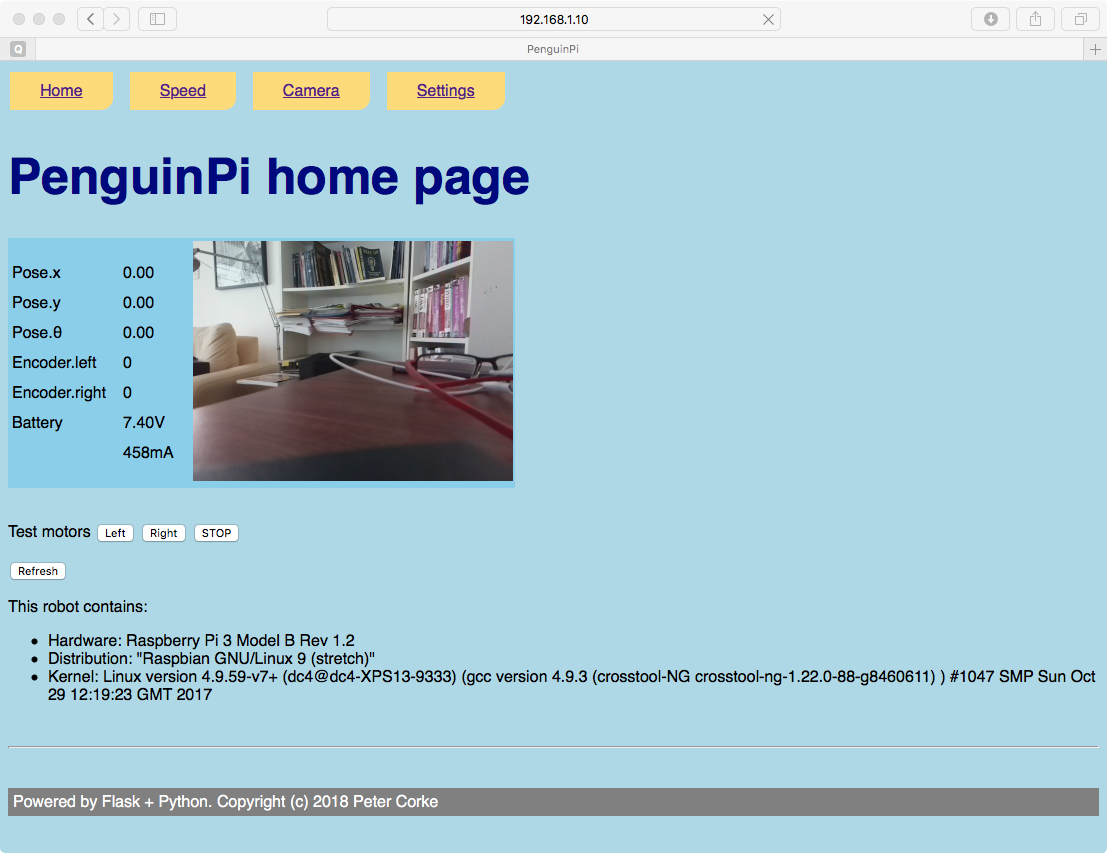
\includegraphics[width=0.8\textwidth]{homepage.png}
\caption{Home page}\label{fig:homepage}
\end{figure}

\subsection{Boot process}
At boot time a startup script is run via \texttt{crontab} which is edited by \texttt{sudo crontab -e}
\begin{Code}
@reboot bash /home/pi/.startup-servers.sh
#* * * * * bash /home/pi/check_network.sh
\end{Code}
The first line invokes a hidden script in the user \text{pi}'s home directory which invokes the servers to run at boot time.
This used to be separate motor and camera servers, but is now just the \texttt{ppweb.py} server.

The second line, commented out, used to run the IP network update daemon every minute.  That functionality is now 
subsumed by the \texttt{ppweb.py} server.


%%%%%%%%%%%%%%%%%%%%%%%%%%%%% WEB SERVER
\subsection{Web API}
A light-weight web server written using the Flask Python package and is built on the Python API.
It implements  a human-friendly interface to the robot, see Figure \ref{fig:homepage}  as well as a
 RESTful programmatic interface. 
This interface  makes the PenguinPi robot into a network resource which can be controlled
 by any computer on the same network.
 
 In order to use this we must first determine the robot's IP address which is usually assigned by a DHCP server (this depends on its network configuration defined by \texttt{/etc/network/interfaces}).  
 The IP address is displayed on the OLED some time after the Raspberry Pi
has booted.
The web server can be accessed on port 8080 at the robot's IP address.  The home page shows all relevant robot status including 
a snapshot from the robot's camera, encoder values, dead-reckoned pose, battery voltage, motor testing, Raspberry Pi hardware and software details. 
Additional pages, accessible via the navigation bar, allow motor speed setting and camera parameter adjustment.
All pages can be automatically refreshed by adding the query \texttt{?refresh=N} where N is the refresh interval in seconds.

The robot's pose is estimated on board by a thread that performs dead reckoning.  It reads the encoder values at 10\unit{Hz} (default value) and using knowledge of wheel
diameter and wheel separation (distance between the middle of the tyres is used).


Commands are implemented by access to the URLs given in Table \ref{tab:api-xref}.  In addition some higher level functions are provided

\begin{tabular}{|l|l|l|l|} \hline
Operation & URL & Query & Return \\\hline\hline
Set velocity & \texttt{/robot/set} & \texttt{?vel=LEFT,RIGHT} & state \\
 &                      & \texttt{?time=DURATION}  & state\\
 &                      & \texttt{?acc=DURATION} & state \\
Get state & \texttt{/robot/get/state} & & state \\
Set state & \texttt{/robot/set?state=X,Y,TH} && \\ \hline
Get image & \texttt{/robot/camera/get} & & image \\
 & &                  \texttt{?resolution=(WIDTH,HEIGHT)} & image \\
 &  &                 \texttt{?awb=AWB} & image\\\hline
\end{tabular}

where state is a JSON message that contains odometry and onboard dead reckoned pose.
The image is returned in PNG format.

If a time is specified, second argument, the motors are set to the desired velocities and after the specified interval the velocities are set to zeros.  All timing done on the Raspberry Pi
and this is a blocking command, it returns when the time period has elapsed.
If acceleration is specified, third argument, the speed ramps up linearly over the acceleration period, and ramps down at the end.  The total motion time is given by the time 
parameters which must be greater than twice the acceleration time.
The displacement for each wheel is $V (T - T_a)$.


TODO: Commands to read the error log.  Command to write string to the OLED.

\subsection{MATLAB API}
The original MATLAB API used sockets to communicate with a Python-based server on the \rpi\ with a bespoke string-based protocol.
By comparison accessing the web API from MATLAB is very easy
\begin{Code}
webread('http://10.0.0.1/set/motor', 'speed', [20 -30], 'time', 5)
\end{Code}
The \texttt{webread} function automatically converts numeric values to strings, and turns vectors into comma separated lists.

\fvset{formatcom=\color{blue},fontseries=c,fontfamily=courier,fontsize=\small}

A connection to the robot is established by creating an instance of a \var{PiBot} object
\begin{Code}
>> pibot = PiBot('131.72.14.7')
\end{Code}
which is passed a string with the robot's IP address.  This object has a number of methods:

\begin{tabular}{|l|p{3cm}|} \hline
MATLAB command & Purpose \\ \hline\hline
\var{stop()} & Stop all motors \\
\var{state = setMotorVelocity(left, right)} & Velocities given as 2 arguments \\
\var{state = setMotorVelocity([left right])} & Velocities given as 2-element vector \\
\var{state = setMotorVelocity([left right], time)}& Specify total motion time\\
\var{state = setMotorVelocity([left right], time, acc)} & Specify time and acceleration time\\ \hline
\var{img = getCameraImage()} & Get image from camera \\ \hline
\var{setLED(led, state)} & Set LED (2-4) to logical value \\
\var{pulseLED(led, time)} & Pulse LED (2-4) for integer milliseconds \\
\var{n = getButtonCount()} & Get user button presses (and reset) \\
\var{sendText(str)} & Send string to OLED display \\ \hline
\end{tabular}

\var{state} is a structure that contains current encoder values and dead-reckoned robot configuration.  For example:
\begin{Code}
>> pibot.setMotorVelocity(20, -20)
>> pause(2)
>> pibot.stop()
\end{Code}

\bibliographystyle{IEEEtran}
\bibliography{refs}

\newpage
\appendix
\section{Complete command list}
A complete list of all commands accessible through the low-level serial API, Python API and web API are given in Table \ref{tab:api-xref}.
The implementation of each API call on the robot can be found by searching
for the PPI opcode in the file \texttt{datagram.c}.
The symbolic names of the virtual devices on the PPI are listed in Table \ref{tab:devices}.


\DefineShortVerb{\+}


\fvset{formatcom=\color{black},fontseries=c,fontfamily=courier,fontsize=\small}

\begin{table}[h]
\centering
\begin{tabular}{|l|l|} \hline
Address & Purpose \\ \hline\hline
+AD_ADC_C+ & ADC current channel \\
+AD_ADC_V+ & ADC current channel \\ \hline
+AD_HAT+ & HAT board \\ \hline
+AD_LED_R+ & LED1 red \\
+AD_LED_G+ & LED1 green \\
+AD_LED_B+ & LED1 blue \\
+AD_LED_2+ & LED2 \\
+AD_LED_3+ & LED3 \\
+AD_LED_4+ & LED4 \\ \hline
+AD_MOTOR_L+ & left wheel motor \\ 
+AD_MOTOR_R+ & right wheel motor \\ \hline
+AD_MULTI+ & both motors \\ \hline
+AD_SERVO_A+ & servo channel A \\
+AD_SERVO_B+ & servo channel B \\ \hline
\end{tabular}
\caption{Symbolic names for device addresses}\label{tab:devices}
\end{table}



\fvset{formatcom=\color{black},fontseries=c,fontfamily=courier,fontsize=\tiny}

\begin{landscape}
\setlength\LTcapwidth{\linewidth}
\begin{longtable}{|l|l|l|l|p{5cm}|}\hline
PPI Opcode &                         Python method &      Web call & Argument & Purpose \\ \hline\hline
+ADC_GET_POLE+ &           +get_pole+ &      +/adc/get/pole?chan=N+                           & +float+ & Get z-plane pole  \\
+ADC_GET_SCALE+ &         +get_scale+ &    +/adc/get/scale?chan=N+                          & +float+ & Get scale factor \\
+ADC_GET_SMOOTH+ &     +get_smooth+ & +/adc/get/smooth?chan=N+   & +float+ & Get filtered value  \\
                                        &                              & +/battery/get/voltage+ & +float+ & Get battery voltage (filtered) \\
                                        &                              & +/battery/get/current+ & +float+ & Get battery current (filtered) \\
+ADC_GET_VALUE+ &         +get_value+   &   +/adc/get/value?chan=N+                          & +float+ & Get unfiltered value \\ \hdashline
+ADC_SET_POLE+ &           +set_pole+ &       +/adc/set?chan=N&pole=P+                        & +float+ & Set z-plane pole  \\
+ADC_SET_SCALE+ &         +set_scale+ &        +/adc/set?chan=N&scale=S+                     & +float+ & Set scale factor \\ \hline
+HAT_GET_BUTTON+ &      +get_button+ & +/hat/button/get+     & +uint8+ & Get number of button 4 presses since last read \\
+HAT_GET_DIP+ &               +get_dip+ & +/hat/dip/get+               & +uint8+ & Get value of DIP switch \\
+HAT_GET_LEDARRAY+ &  +get_ledarray+ & +/hat/ledarray/get+   & +uint16+ & Get value of LED array \\ \hdashline
+HAT_SET_IP_ETH+ &         +set_ip_eth+ &                         & +uint32+ &Set eth IP address on OLED \\
+HAT_SET_IP_WLAN+ &      +set_ip_wlan+ &                       & +uint32+ & Set wlan IP address on OLED\\
+HAT_SET_LEDARRAY+ &   +set_ledarray+ & +/hat/ledarray/set?value=L+    & +uint16+ & Set value of LED array\\
+HAT_SET_SCREEN+ &       +set_screen+ & +/hat/screen/set?value=S+     & +uint8+ & Select OLED information screen \\ \hline
+LED_GET_STATE+ &          +get_state+ &    +/led/get?led=L+                                  & +uint8+ & Get state of LED \\
+LED_SET_COUNT+ &         +set_count+ & +/led/set/count?id=L&value=N+  & +uint8+ & Turn LED on for interval \\
+LED_SET_STATE+ &           +set_state+ & +/led/set/state?id=L&value=N+   & +uint8+ & Set LED state (0 or 1)\\ \hline
+MOTOR_GET_CONTROL_MODE+ &  &  & & Get motor control mode \\
+MOTOR_GET_ENC+ &   +get_encoder+ &       +/motor/get/encoder?id=N+           & +uint16+ & Get motor encoder value \\
+MOTOR_GET_ENC_MODE+ & +get_encoder_mode+ &    +/motor/get/enc_mode?id=N+     & +int8+ & Get motor encoder mode \\
+MOTOR_GET_KVI+ &  +get_kvi+ &   +/motor/get/kvi?id=N+     &  +int16+ & Get  velocity loop integral gain  \\
+MOTOR_GET_KVP+ & +get_kvp+ &       +/motor/get/kvp?id=N+       & +int16+ & Get  velocity loop position gain  \\
+MOTOR_GET_VEL+ & +get_velocity+ &    +/motor/get/vel/id=N+   & +int8+ & Get  velocity setpoint \\ \hdashline
+MOTOR_SET_CONTROL_MODE+ & &&&  Set motor control mode\\
+MOTOR_SET_ENC_MODE+ & +set_encoder_mode+&                                     & +uint8+ & Set motor encoder mode \\
+MOTOR_SET_ENC_ZERO+ & &                                    & & Set  encoder to zero \\
+MOTOR_SET_KVI+ & +set_kvi+ &    +/motor/set/kvi?value=V&id=N+        & +int16+ &Set  velocity loop integral gain  \\
+MOTOR_SET_KVP+ & +set_kvp+ &   +/motor/set/kvp?value=V&id=N+          &  +int16+ & Set  velocity loop position gain   \\
+MOTOR_SET_VEL+ & +set_velocity+ &  +/motor/set/velocity?value=V&id=N+  & +int8+ & Set  motor velocity setpoint \\ \hline
+MULTI_ALL_STOP+ & +set_allstop+ & +/robot/stop+             & & Stop all motors \\
+MULTI_CLEAR_DATA+ & &                                              & & Stop motors, zero encoders \\
+MULTI_GET_ENC+ & +get_encoders+ &                 & +uint16[2]+ & Get both encoders \\
+MULTI_SET_VEL+ & +set_velocity+ &                              & +int8[2]+ & Set both motor speeds \\
+MULTI_SET_VEL_GET_ENC+ & +setget_velocity_encoders+ & +/robot/set/velocity?value=L,R&acc=A&time=T+  & +int8[2], uint16[2]+ & Set both motor speeds, get both encoders  \\ \hline
+SERVO_GET_MAX_PWM+ & +get_PWM_range+ & & +int16+ & \\
+SERVO_GET_MAX_RANGE+ & +get_range+ & & +int16+ & \\
+SERVO_GET_MIN_PWM+ & +get_PWM_range+ & & +int16+ & \\
+SERVO_GET_MIN_RANGE+ & +get_range+ & &  +int16+ & \\
+SERVO_GET_POSITION+ & +set_position+ & & +int16+ & Get position of servo \\
+SERVO_GET_STATE+ & +get_state+ & & +uint8+ & \\ \hdashline
+SERVO_SET_MAX_PWM+ & & & &  \\
+SERVO_SET_MAX_RANGE+ & +set_range+ & & +int16+ & Set maximum position \\
+SERVO_SET_MIN_PWM+ &  & & &                                     \\
+SERVO_SET_MIN_RANGE+ & +set_range+ &             & +int16+ & Set minimum position \\
+SERVO_SET_POSITION+ & +set_position+ &                 & +int16+ & Set position of servo \\
+SERVO_SET_STATE+ & +set_state+ & & +uint8+ &\\  \hline
\caption{Relationship between PenguinPi opcodes, Python API method name and web API URL.}\label{tab:api-xref}
\end{longtable}
\end{landscape}


%Set speed & MOTOR\_SET\_SPEED & set\_speed(v) & /motor?speed=sl,sr \\
%Get encoder & MOTOR\_GET\_ENCODER & set\_speed(v) & /motor \\
%
%Control LED & LED\_SET\_STATE & set\_state(v) & /led?[RGB234]=[01] \\
%Pulse LED & LED\_SET\_COUNT & set\_count(v) & /led?[RGB234]=[01] \\
%Set array & LED\_SET\_ARRAY & set\_array(v) & /led?array=val \\ 
%Send string to OLED & & send\_string(s) & /display?disp=s \\
%User button & ALL\_GET\_BUTTON & wait\_button() & \\
%\end{tabular}
%


\UndefineShortVerb{\+}
\fvset{formatcom=\color{blue},fontseries=c,fontfamily=courier,xleftmargin=4mm,commentchar=!}


\section{Recent changes to the code base}

There were a number of limitations within the initial code base:
\begin{enumerate}
\item The TC2 overflow interrupt occurs every 12.8\us.  The high rate imposes a very significant computational load as well as being
an inconvenient unit of time.

\item The motor speed is at least 20\% less than commanded.  

\item The motor control exhibits  \textit{grittyness} which was likely due to control jitter.  

\item Random premature triggering of timers and bad encoder values.

\item Occasional and random data communications errors, particularly at high datagram rates.  

\item An error  occurred consistently every time the IP address update daemon ran.

\item The worst case loop time, well over 20\ms, introduces a signifcant latency on the response time for datagrams.  

\item The datagram logic requires that every GET function has a corresponding SET function which is nonsensical in many cases.
Maintaining consistency of opcodes between the PPI and Python code is problematic.


\item The original MATLAB-Python with a bespoke string-based protocol was difficult to extend, treated images inefficiently, and gave little information about the robot state to the student without having to write code.

\end{enumerate}

Numerous changes were implemented to address these limitations:
\begin{enumerate}

\item Change the main clock interrupt period to 1\ms\ instead of 12.8\us.  This is achieved by using timer TC1 which was freed up by eliminating brightness control of the RGB LEDs which not a useful UI feature.  This also frees up TC2 which could be used to control
two servo channels.  TC1, clocked at 20\unit{MHz} can also be used to make precision timing measurements, see \texttt{timer\_get()}.

\item This was the result of the control interval (250 loops) being 20\% longer
than the 20\ms\ assumed in the code.  This is largely due to interrupt burden, from the TC2 interrupts mentioned above. Additional instrumentation indicates the actual interval was 23.8\ms\ but it increases with motor speed due to the increased CPU load from encoder interrupts.  With one wheel turning at speed 100 the interval increases to 27\ms. 
The motor control loop now occurs in the millisecond interrupt handler but with interrupts enabled, ie. it executes on the interrupt stack.
This ensures accuracy of the control interval. 

\item Analysis shows that the control loop interval is quite variable, in particular
the OLED refresh (every 1000 loops) takes around 15\ms\ compared to the normal 0.1\ms\ loop time.
To a lesser extent it is also impacted by datagrams received, and button presses.
The estimated velocity is simply computed between calls which assumes that this time is constant.
This implies that the assumed sampling time is incorrect.  A longer control interval makes the estimated velocity higher (more encoder ticks accumulate over the longer interval) so the controller will
reduce motor speed.

Change 2 also eliminates the control jitter and the motors run much more quietly.
The OLED is also updated more periodically in the polling loop, triggered by a counter updated by the millisecond interrupt handler.  

\item A number of counters (for time and encoders) are implemented as 16-bit integers that are modified in the timer overflow interrupt handler and tested or reset by non-interrupt code.  This is unsafe
and declaring the variables as volatile is not sufficient.  Operations in the non-interrupt code must be performed with interrupts disabled using the \texttt{ATOMIC} macro.  With slower timer interrupts, many counters are now 8 bit instead of 16 bit which means that updates are atomic.  All  counters $> 8$ bit
are now protected by \texttt{ATOMIC} macros.

\item Several design issues were addressed:
\begin{itemize}
\item Datagram receive code did not test the UART for data availability and relied on a fixed delay which assumed no inter-character gap.
Datagram serial receive now polls the UART for data every 20\us\ upto a maximum timeout period.
\item Mutex to prevent multiple Python threads simultaneously communicating with the PPI, has  resolved long-standing subtle data communications bugs and performance is now error free, even with very high
levels of traffic.
\end{itemize}

\item Several design issues were addressed:
\begin{itemize}
\item A missing switch break meant that OLED update ``fell through'' into the ADC code generating an error.  
\item The IP address update daemon opens the serial port and its instance of \texttt{penguinPi.py}  steals incoming bytes from the control process, leading to a reasonable
number of failed read requests. An updated version of PySerial has been installed which supports exclusive access to the serial port --
preventing the IP address update daemon running when a control process is running.
\end{itemize}  

\item The latency has been reduced by:
\begin{enumerate}
\item modifying the OLED screen update logic to one memory block per polling loop, instead of all 16 in one polling loop.
\item removing the high rate clock overflow interrupt.
\end{enumerate}

\item The datagram logic has been rewritten so that a GET command returns the GET opcode, not the corresponding SET opcode.  This allows nonsensical SET codes to be eliminated. All GET codes have their top-bit set.
The datagram defines were rewritten as \texttt{enums}, rather than \texttt{\#define}s to ensure that there can be no value clash, and \texttt{defines.py} parses the
datagram definitions in \texttt{datagram.h} and creates a Python pickle file \texttt{atmel-symbols.pickle} imported by \texttt{penguinPi.py}.

\item A webserver on the robot provides a unified user and programmatic interface to the robot, and is easily extensible.

\end{enumerate}

Other significant changes compared to PenguinPi 2018 include:
\begin{itemize}
\item Refactoring of code, greater use of \texttt{varargs}, attributes and \texttt{setjmp/longjmp} for error handling.  All code relating to degrees and angle PID control removed.
\item Code is now split across 6 files written in pseudo-OO format.  Each \texttt{module.c} has a corresponding \texttt{module.h} and any
exported functions or variables are prefixed with \texttt{module\_}.  Each  \texttt{module.h} uses preprocessor conditionals to prevent multiple inclusion.

\item ADC conversions are now initiated by the millisecond interrupt handler, eliminating jitter and allowing a simple digital filter to be implemented.
\item IP addresses were set using one opcode per digit with a 16-bit payload, yet an IP address is simply a 32-bit number.
 IP addresses are set using a single opcode with a 32-bit payload.
\item The CRC polynomial 0xAE is not optimal for small packet sizes.  
\cite{Koopman04} and \cite{Koopman} suggests that for messages in the range 32 to 64 bits the optimal polynomial is 0x97, and this change
has been made to the PPI and Python code.  
\item The start byte is not unique and byte stuffing should be implemented, or
introduce a 2-byte start sequence. The start byte
runs the risk of collision with data, and this could be reduced by making a 2-byte sequence or byte stuffing, the latter is more complex.  With judicious choice of address and commands, the risk of start byte collision is just with the payload so in the worst case their would be
four bytes stuffed into the packet.
The start byte issue does not appear to be a problem in practice.

\item A builtin web server using Flask, see Section \ref{sec:flask}, which allows user and programmatic control of the robot
\item On board pose estimation by dead reckoning from encoder velocity
\item OLED interface improvements:
\begin{itemize}
\item The ability for a user program to display text on the OLED display
\item Additional information screens on the OLED: timing details, last datagram, user text etc.
\item Use of inverse text (black on white) to make the OLED display more readable
\item Some screens use button 3 to perform an action, ie. zero encoders from the encoder screen
\item The OLED screen color is inverted when the battery voltage is low.
\end{itemize}
\item Motor state and control structures have been merged.
\item Consistently change motor A and B notation to R and L respectively.
\end{itemize}
See the git log for more details.  %Overall the code has reduced slightly from 2856 LOC to 2786 LOC.  Active lines of code, comments??

\section{Desirable hardware changes}
\begin{itemize}
\item Power related:
 \begin{itemize}
 \item Fix the charging connector, it detaches from the board too easily
 \item Recharge battery and operate the robot at the same time
 \item Can we charge the battery from a standard USB port, rather than special charger?
 \end{itemize}
\item Hat related:
\begin{itemize}
 \item Add a header on the hat that allows easy prototyping using hat i/o signals (and Vcc), eg. ribbon connection to a prototyping board (and somewhere to put it).
 \item Add standard 3 pin headers for servo motors connected to timer 1/2 OCP
 \item Add a header for switched DC supply driven by a GPIO from Raspberry Pi or Atmel.
\end{itemize}
\item Fix the placement of the second Hall-effect sensor to enable quadrature operation
\item Use an omni-polar Hall-effect sensor to double the encoder resolution
\end{itemize}

\section{Random notes}
\begin{itemize}
\item Login credentials are pi/PenguinPi.
\item Network settings: \texttt{sudo vi /etc/network/interfaces}
\item Check interfaces: \texttt{ip address show}
\item Automatic process startup: \texttt{sudo crontab -e}
\item Boot-time process start is handled by \texttt{/home/pi/.startup-servers.sh}
\item We disable the RPi builtin WiFi by a line in \texttt{/boot/config.txt}
\begin{Code}
  dtoverlay=pi3-enable-wifi
\end{Code} 
\end{itemize}


\section{Schematics}
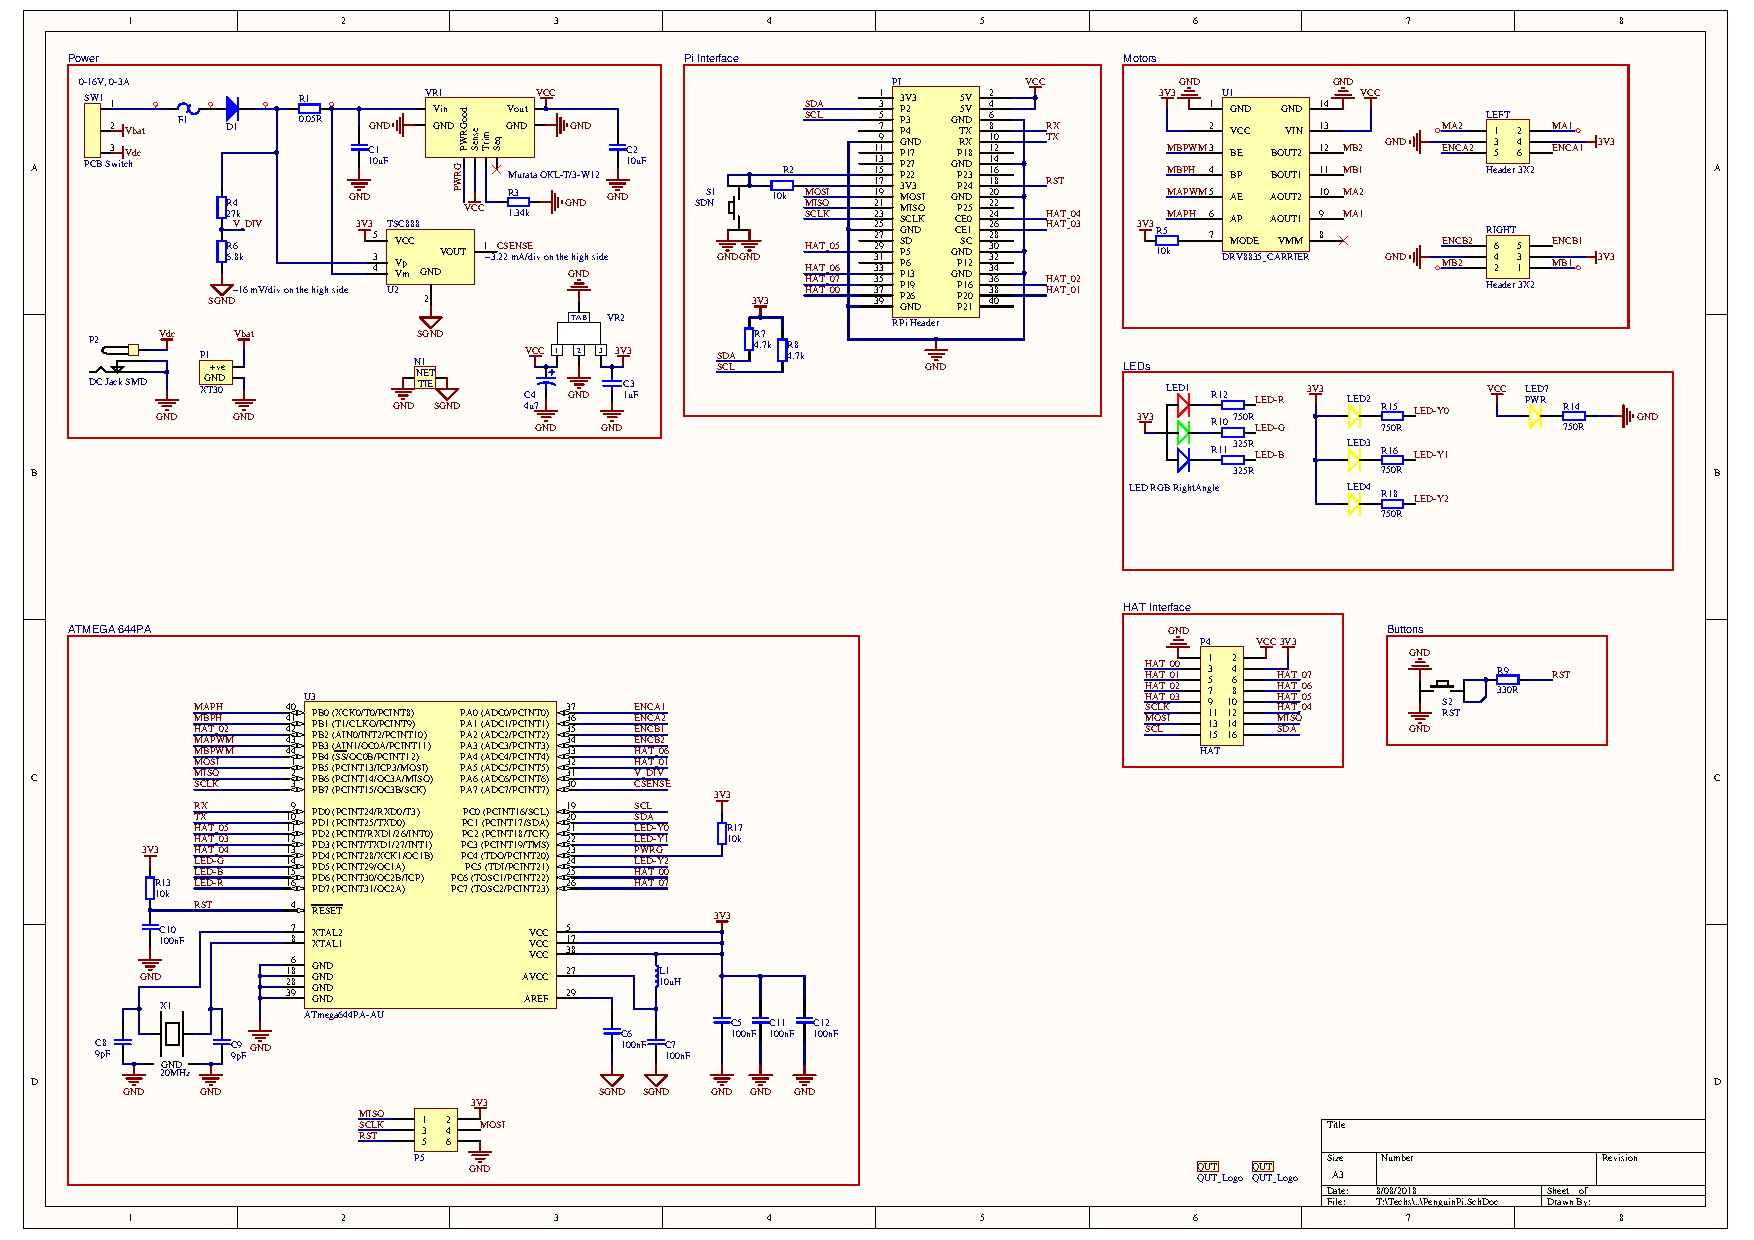
\includepdf[pages=-,landscape,pagecommand={},width=1.4\textwidth]{schematics/PenguinPi.pdf}

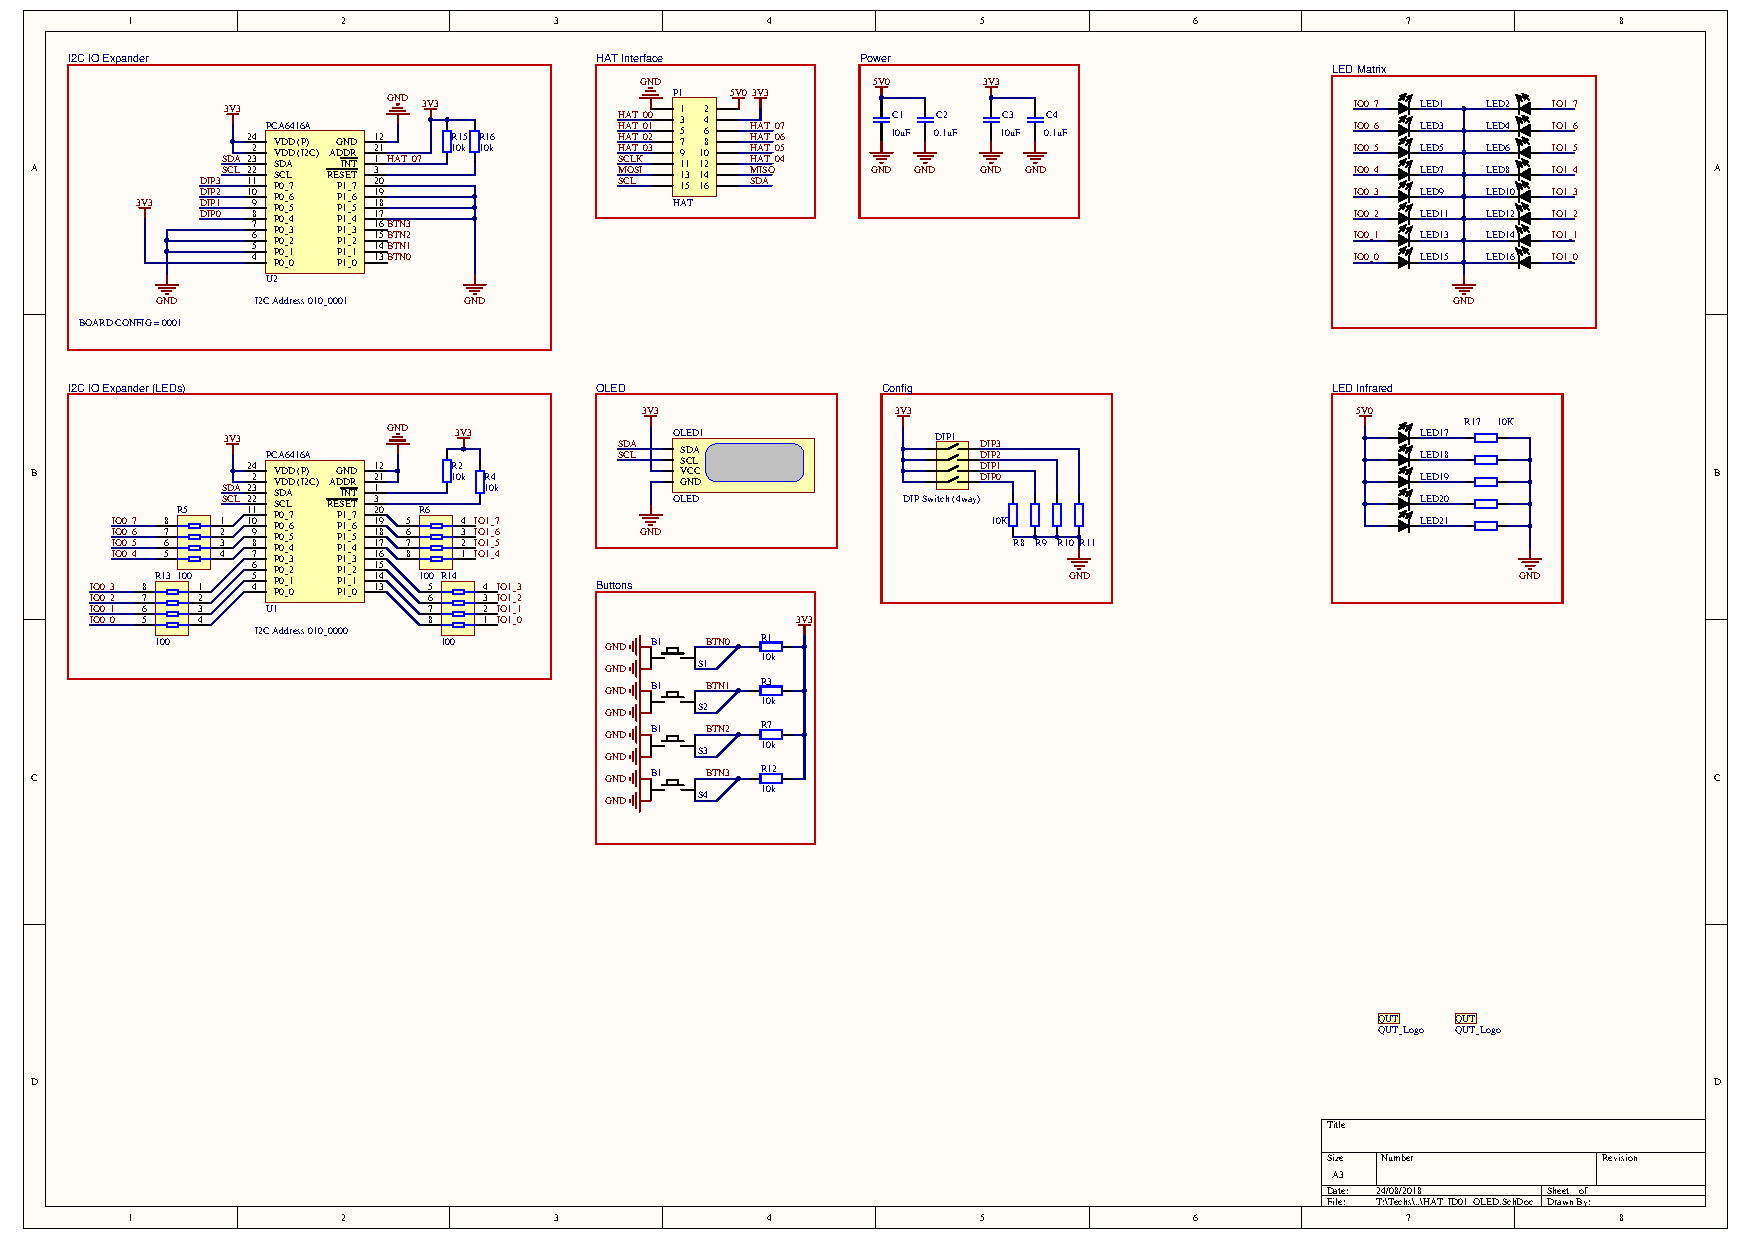
\includepdf[pages=-,landscape,pagecommand={},width=1.4\textwidth]{schematics/HAT_ID01_OLED.pdf}


\end{document}
